\documentclass[]{book}
\usepackage{lmodern}
\usepackage{amssymb,amsmath}
\usepackage{ifxetex,ifluatex}
\usepackage{fixltx2e} % provides \textsubscript
\ifnum 0\ifxetex 1\fi\ifluatex 1\fi=0 % if pdftex
  \usepackage[T1]{fontenc}
  \usepackage[utf8]{inputenc}
\else % if luatex or xelatex
  \ifxetex
    \usepackage{mathspec}
  \else
    \usepackage{fontspec}
  \fi
  \defaultfontfeatures{Ligatures=TeX,Scale=MatchLowercase}
\fi
% use upquote if available, for straight quotes in verbatim environments
\IfFileExists{upquote.sty}{\usepackage{upquote}}{}
% use microtype if available
\IfFileExists{microtype.sty}{%
\usepackage{microtype}
\UseMicrotypeSet[protrusion]{basicmath} % disable protrusion for tt fonts
}{}
\usepackage[margin=1in]{geometry}
\usepackage{hyperref}
\hypersetup{unicode=true,
            pdftitle={Competitor Scale and Mutual Fund Behavior},
            pdfauthor={Laszlo Jakab},
            pdfborder={0 0 0},
            breaklinks=true}
\urlstyle{same}  % don't use monospace font for urls
\usepackage{natbib}
\bibliographystyle{apalike}
\usepackage{longtable,booktabs}
\usepackage{graphicx,grffile}
\makeatletter
\def\maxwidth{\ifdim\Gin@nat@width>\linewidth\linewidth\else\Gin@nat@width\fi}
\def\maxheight{\ifdim\Gin@nat@height>\textheight\textheight\else\Gin@nat@height\fi}
\makeatother
% Scale images if necessary, so that they will not overflow the page
% margins by default, and it is still possible to overwrite the defaults
% using explicit options in \includegraphics[width, height, ...]{}
\setkeys{Gin}{width=\maxwidth,height=\maxheight,keepaspectratio}
\IfFileExists{parskip.sty}{%
\usepackage{parskip}
}{% else
\setlength{\parindent}{0pt}
\setlength{\parskip}{6pt plus 2pt minus 1pt}
}
\setlength{\emergencystretch}{3em}  % prevent overfull lines
\providecommand{\tightlist}{%
  \setlength{\itemsep}{0pt}\setlength{\parskip}{0pt}}
\setcounter{secnumdepth}{5}
% Redefines (sub)paragraphs to behave more like sections
\ifx\paragraph\undefined\else
\let\oldparagraph\paragraph
\renewcommand{\paragraph}[1]{\oldparagraph{#1}\mbox{}}
\fi
\ifx\subparagraph\undefined\else
\let\oldsubparagraph\subparagraph
\renewcommand{\subparagraph}[1]{\oldsubparagraph{#1}\mbox{}}
\fi

%%% Use protect on footnotes to avoid problems with footnotes in titles
\let\rmarkdownfootnote\footnote%
\def\footnote{\protect\rmarkdownfootnote}

%%% Change title format to be more compact
\usepackage{titling}

% Create subtitle command for use in maketitle
\newcommand{\subtitle}[1]{
  \posttitle{
    \begin{center}\large#1\end{center}
    }
}

\setlength{\droptitle}{-2em}
  \title{Competitor Scale and Mutual Fund Behavior}
  \pretitle{\vspace{\droptitle}\centering\huge}
  \posttitle{\par}
  \author{Laszlo Jakab}
  \preauthor{\centering\large\emph}
  \postauthor{\par}
  \predate{\centering\large\emph}
  \postdate{\par}
  \date{March 11, 2018}

\usepackage{booktabs}
\usepackage{longtable}
\usepackage{array}
\usepackage{multirow}
\usepackage[table]{xcolor}
\usepackage{wrapfig}
\usepackage{float}
\usepackage{colortbl}
\usepackage{pdflscape}
\usepackage{tabu}
\usepackage{threeparttable}
\usepackage[normalem]{ulem}

\usepackage{amsthm}
\newtheorem{theorem}{Theorem}[chapter]
\newtheorem{lemma}{Lemma}[chapter]
\theoremstyle{definition}
\newtheorem{definition}{Definition}[chapter]
\newtheorem{corollary}{Corollary}[chapter]
\newtheorem{proposition}{Proposition}[chapter]
\theoremstyle{definition}
\newtheorem{example}{Example}[chapter]
\theoremstyle{definition}
\newtheorem{exercise}{Exercise}[chapter]
\theoremstyle{remark}
\newtheorem*{remark}{Remark}
\newtheorem*{solution}{Solution}
\begin{document}
\maketitle

{
\setcounter{tocdepth}{1}
\tableofcontents
}
\hypertarget{abstract}{%
\chapter*{Abstract}\label{abstract}}
\addcontentsline{toc}{chapter}{Abstract}

I study the effects of competition on the investment behavior and
performance of active mutual funds. I find that funds respond to
increased competitor scale by curtailing costly active management. To
establish causality, I exploit quasi-exogenous variation in fund flows
created by a natural experiment---the 2003 mutual fund scandal. Funds
whose competitors were the most affected by the scandal expand active
management and perform better after the scandal. Interpreting the
findings through the lens of models of decreasing returns to scale
indicates information asymmetry between fund managers and outside
investors.

\hypertarget{introduction}{%
\chapter{Introduction}\label{introduction}}

What is the impact of competition on the allocation of capital inside
firms? In general, competition affects both a firm's efficient scale and
the optimal composition of its investments. In the case of mutual funds,
managers choose the composition of investments, while outside investors
determine the capital allocated to the firm. I exploit changes in the
size of competing funds to identify the effect of competition on capital
allocation. I demonstrate that funds respond to competition by
reallocating capital from costly active strategies to cheaper, more
passive portfolios. I address endogeneity concerns by investigating a
natural experiment created by the 2003 mutual fund scandal. Fund
families engulfed by the scandal were penalized by investor outflows,
which I exploit as quasi-exogenous variation in competitor size. I show
that close competitors of affected funds increased active management,
and reaped improved performance following the scandal.

My findings shed light on a key tension that occurs when mutual funds
face decreasing returns to scale. As competition eliminates investment
opportunities, the fund's optimal response is to reallocate capital
toward passive portfolios. However, if investors are symmetrically
informed, they withdraw capital from the fund \citep{bg04}. Decreased
fund size lowers the marginal cost of active management, countervailing
the shift toward passivity. In models of fund behavior, the size effect
dominates in equilibrium, predicting increased capital allocated to
active strategies in response to competition \citep{pst17L}.
Interpreting my findings in this framework points to information
asymmetry between funds and outside investors resulting in mismatch
between investment opportunities and capital that is not fully undone by
the firm's actions \citep{bbl17}. This interpretation also provides a
potential explanation for the observed relation between measures of
activeness such as active share \citep{cp09} or industry concentration
\citep{ksz05} and future fund performance: if managers have private
information about investment opportunities, their actions carry
information about expected returns.

\citet{ps12} argue that each fund's investment opportunities become less
lucrative as the size of competing funds increases. Decreasing returns
to competitor scale are grounded in liquidity constraints and the
associated price impact of other funds' trades. Consider a skilled fund
receiving signals of the fundamental value of securities. In the absence
of competitors, the limiting factor of the fund's profits is the price
impact of its own trades. Introducing another fund that receives
correlated signals is detrimental to the fund's profitability. Since
both funds chase similar investments, either one might be first to
invest in a particular opportunity, pushing up its price. The total
impact of the other fund will depend on both the similarity of its
signals, which determines the likelihood of being leapfrogged, and the
fund's size, which governs the magnitude of price impact. Competitor
size is therefore the sum of the product of similarity and fund size
across all potential competitors: \[
\text{Competitor Size}_i = \sum_{j\neq i} \text{Similarity}_{i,j} \times \text{Fund Size}_j.
\] If funds receive identical signals, similarity equals one, and
competitor size will equal aggregate industry size
\citep{pst15}.\footnote{
I measure fund similarity by the cosine similarity of market capitalization adjusted portfolio weights. I cap adjust portfolio weights by dividing them with market weights, as cross-holdings of small-capitalization stocks are more informative of similarity than cross-holdings of large capitalization stocks [@ccp05].
} Unlike industry size, competitor size is specific to each fund, which
allows for studying variation in the cross-section. Most importantly,
taking fund similarity into account enables me to analyze novel evidence
on decreasing returns to competitor scale from a natural experiment.

\citet{bg04} posit a relation between active share and fund size and
fees. \citet{pst17L} introduce a richer model of fund behavior,
proposing that funds jointly optimize turnover and portfolio liquidity.
Portfolio liquidity is a multi-dimensional object that can be decomposed
as a product of stock liquidity and diversification (itself a product of
coverage and balance). I make the model-driven argument that if
investors do not fully recognize the detrimental impact of competition
on future returns, then increases in competitor size will have a
measurable impact on fund activeness even conditional on own size, fees,
and time fixed effects.

My empirical analysis is based on a sample of actively managed U.S.
equity funds spanning 1980-2014, with size and returns information from
CRSP linked to Thomson Reuters holdings data. Guided by theory, I relate
quarterly changes in competitor scale to changes in active share,
turnover to portfolio liquidity ratio, and various components of
portfolio liquidity, conditional on own size, expense ratio, and time
fixed effects. I find that funds react to increases in competitor scale
by decreasing active share and increasing all dimensions of portfolio
liquidity.

I bolster the causal link between competitor scale, fund behavior, and
performance by providing novel evidence from a natural experiment
created by the 2003 mutual fund scandal. In September 2003, the New York
State Attorney General announced investigations into illegal trading
practices at several prominent mutual fund families. As investigations
gained momentum, evidence mounted that families had allowed favored
clients to abuse ordinary investors by trading fund shares at stale
prices \citep{zitzewitz06}. By October 2004, a total of twenty-five fund
families were embroiled in the scandal \citep{hw05}. The involved
families represented a considerable proportion of the industry,
collectively managing over a fifth of assets prior to the scandal.
Following the announcement of the investigations, investors abruptly
began withdrawing capital from tainted families
(Figure\textasciitilde{}\ref{fig:scandalFlows}).

I exploit post-scandal outflows at tainted funds as an exogenous shock
to the competitor size of funds pursuing similar investment strategies.
We would expect the favorable impact of lessened competitor scale to be
greatest for the closest pre-scandal competitors of tainted funds. Under
the hypothesis of decreasing returns to competitor scale, these funds
experience a comparative improvement in their investment opportunities.
Therefore, we would expect them to increase capital allocation to active
strategies relative to less close competitors of tainted funds, and see
relative improvements in performance. I take two different approaches to
testing these hypotheses, both of which confirm decreasing returns to
competitor scale and the associated fund response.

Since involved funds are directly affected by the scandal, I identify
decreasing returns to competitor scale by comparing outcome paths at
untainted funds. The first approach compares pre- and post-scandal
outcomes as a function of pre-scandal exposure to competition from
tainted funds. I measure exposure by the fraction of competitor scale in
August 2003 accounted for by prospective tainted families. The
competitor size of high exposure funds decreased significantly more
during the scandal. Consistent with comparatively improved investment
opportunities, high exposure funds increased active share and decreased
portfolio liquidity relative to low exposure funds, and experienced
comparatively better performance. Statistical tests show no evidence of
differential trends by scandal exposure in the pre-period.

The second approach links fund outcomes directly to abnormal outflows at
tainted funds. I use a linear model to decompose post-scandal flows at
involved funds between time variation common to all funds and abnormal
flows attributable to scandal involvement. I show that untainted funds
whose tainted competitors experienced greater abnormal outflows saw
relative declines in competitor size, improvements in performance, and
shifted to more active portfolio management. Variation in competitor
size attributable purely to abnormal outflows is negatively related to
both fund performance and activeness, providing direct
quasi-experimental evidence of decreasing returns to competitor scale.

The picture which emerges from these analyses is one in which portfolio
managers optimize investment behavior in real time as they respond to
fluctuations in investment opportunities that are not immediately
apparent to outside investors. Such a world seems sensible. It is
unlikely that retail investors pay the same level of attention to market
developments as professional portfolio managers. Fund managers make
trading decisions based on their perception of investment opportunities
on a daily basis. Since they have more short-term flexibility over
trading than over fund expense ratios, it makes sense that their
portfolio allocation decisions would serve as an important dimension of
optimizing behavior. This interpretation is also consistent with recent
evidence from the literature on fund optimizing behavior in the face of
time-varying investment opportunities. \citet{knv16} argue that mutual
funds allocate attention optimally between factor timing and stock
picking as the nature of opportunities varies over the business cycle.
\citet{pst17} present evidence that funds exploit improved investment
opportunities by increasing turnover.

While the rise of ``closet indexing'' has received much attention and
disapproval, scaling back active management ameliorates the pernicious
effects of decreasing returns to scale, as it brings the costs of active
trading closer in line with decreased benefits. Absent immediate
outflows, deteriorating investment opportunities make a fund ``too
large.'' The fundamental issue might not so much be closet indexing, but
imperfect flows causing mismatch between capital and investment
opportunities.

Studying internal capital markets is difficult due to the dearth of data
on reallocation within firms.\footnote{As \citet{mp13} point out in
  their review, ``Because the study of internal capital markets pertains
  to difficult-to-observe flows within firms, data and measurement
  issues continue to be the focus of recent literature.''} Mutual funds
are a useful testing ground in this respect. Regulation requires funds
to regularly disclose information on capital allocation, size, and
performance. While the organizational simplicity of funds precludes a
study of agency theories of internal capital allocation, the setting is
informative as a neoclassical benchmark.

The rest of the paper proceeds as follows. Section \ref{sec:litReview}
reviews the related literature. Section \ref{sec:model} discusses the
theoretical framework motivating the empirical analyses. Section
\ref{sec:Data} describes the data and the construction of competitor
size. Section \ref{sec:portfolio} presents an empirical analysis of
capital allocation and competitor scale. Section \ref{sec:scandal}
presents evidence from the natural experiment created by the 2003 mutual
fund scandal. Section \ref{sec:conclusion} concludes. The
\href{https://www.dropbox.com/s/qugvhb8b0wqp0cg/LJ_JMP_Data_Appendix.pdf?dl=0}{Data
Appendix} describes in detail the steps in the construction of the
dataset.

\hypertarget{sec:litReview}{%
\chapter{Literature Review}\label{sec:litReview}}

Fund investment behavior has previously been studied in the context of
decreasing returns to own scale. \citet{pw08} investigate the fund
response to inflows. They find that funds diversify in response to new
flows, especially if they operate in relatively illiquid markets.
However, the extent of diversification is small compared to the tendency
to mechanically scale up existing holdings. \citet{pst17L} develop and
test a model of decreasing returns to scale in which size, turnover,
portfolio liquidity, and fund expense ratios are determined jointly in
equilibrium. They show that in the cross-section, larger funds tend to
trade less, cost less, and hold more liquid portfolios, all of which is
consistent with decreasing returns to own scale. However, no paper to
date has examined the impact of competition on fund behavior.

The existing literature has provided evidence of a negative relation
between fund performance and competition. \citet{ww11} find that entry
by similar funds is associated with decreased flows, performance, and
increased exit for incumbents. \citet{pst15} perform a within-fund
analysis showing a negative relationship between performance and
aggregate industry scale. \citet{hkp17} use holdings-based estimates of
fund similarity to measure the number of competing funds, finding that
the number of similar funds is negatively related to both the level and
the persistence of performance in the cross-section. My primary
contribution to this literature is to improve identification by
analyzing evidence from a natural experiment provided by the 2003 mutual
fund scandal. I also provide additional observational evidence that fund
performance is decreasing in competitor scale, especially for funds
pursuing less liquid strategies.

My investigation of fund behavior is informed by models of decreasing
returns to scale by \citet{bg04} and \citet{pst17L}.\footnote{Models of
  decreasing returns to scale rely on the assumption that trading costs
  increase in the size of trades, especially in illiquid securities.
  \citet{bcjt17} provide empirical evidence of such characteristics in
  mutual fund trading costs. Decreasing returns to scale are rooted in
  the price impact of mutual fund trades. Papers presenting evidence on
  price pressure due to mutual fund actions include \citet{cs07},
  \citet{kks12}, \citet{lou12}, \citet{ap14} and \citet{blocher16}. }
Interpreting mutual funds as firms experiencing decreasing returns to
scale in individual investments, my study is related to neoclassical
models of multi-industry firms such as \citet{mp02}.

The preponderance of existing empirical evidence examining fund
performance supports fund level decreasing returns to scale, despite
mixed findings. \citet{chhk04} document decreasing returns to scale
using cross-sectional regressions. \citet{rz15} exploit inflows
following discrete Morningstar ratings changes to study the
size-performance relation in a regression discontinuity framework,
finding little evidence of decreasing returns to scale. \citet*{pst15}
find a negative within-fund association between fund size and
performance, but the economic magnitude of the effect is small, and the
coefficients statistically insignificant when using bias-free estimation
methods. \citet{mclemore16} studies returns following fund mergers,
finding that the increased size of the acquiring fund is accompanied by
decreased performance. In contemporaneous work, \citet{hl17} use a
random effects model and estimate economically significant decreasing
returns to own scale.

In a broad sense, I contribute to a long line of inquiry into the the
nature of skill and constraints among active funds. The typical active
fund fails to generate risk-adjusted returns
\citep{jensen68,malkiel95,malkiel13,gruber96,french08,ff10}. It would
appear at first glance that skill is in short supply among active funds,
a puzzle given the vast resources they manage. However, concurrent poor
performance and large size is consistent with a combination of skill and
decreasing returns to scale \citep*{bg04,ps12}. My analysis gives
additional credence to the existence of economically important
constraints in active management due to decreasing returns to scale. The
empirical results I present are consistent with optimizing behavior by
portfolio managers in the face of evolving constraints in imperfect
capital markets.

\hypertarget{sec:model}{%
\chapter{Theoretical Motivation}\label{sec:model}}

In neoclassical models of capital allocation, firms trade off the
benefit of allocating additional capital to their core competence with
increasing marginal costs due to decreasing returns to scale. Firms
optimally diversify across segments in which they have varying degrees
of skill until marginal costs and benefits are equalized. I motivate my
study by considering the impact of time-varying investment opportunities
(due to competition, for instance) in two such theories of mutual fund
behavior, \citet{bg04}, and \citet{pst17L}.

Consider fund \(i\) managing \(q_{i,t}\) assets in \citet{bg04}. The
fund posts a fixed expense ratio \(f\),\footnote{Following Berk and
  Green, I assume that the fixed expense ratio \(f\) satisfies
  \(f<f^\ast\), where \(f^\ast\) is the expense ratio corresponding to
  profit maximizing fund size \(q^\ast\).} and splits assets between
active and passive management according to \(q_{i,t}=A_{i,t}+P_{i,t}\).
While active management allows the fund to take advantage of positive
NPV investment opportunities in its area of core competence, it also
subjects the fund to quadratic trading costs. I parametrize costs as
\(C(A_{i,t})=\frac{c_t}{M_t}A_{i,t}^2\), where \(A_{i,t}\) is the amount
actively managed, \(M_t\) the size of the market, and \(c_t\) a constant
representing period by period trading costs. Normalizing trading costs
by \(M_t\) implies that price impact per dollar of investment is lower
when total market capitalization is higher. With the normalization, the
model's predictions are in terms of \(FundSize_{i,t}=q_{i,t}/M_t\),
instead of the dollar value of assets under management.

Let \(\mu_{i,t}=E(R_{t+1}\mid R_1,\ldots,R_t)\) be the fund's expected
skill, inferred from publicly available information. In addition,
suppose that the returns to skill depend on time-varying external
factors \(x_{i,t}\), such that expected effective skill is
\(\mu_{i,t}g(x_{i,t})\). \%For convenience, I will later parametrize the
function as the product of baseline skill and competitor size
\(\mu_i(X_{i,t})=\mu_i CompetitorSize^{-\gamma}\). The fund's net alpha
becomes \begin{equation}
\frac{A_{i,t}}{q_{i,t}}\mu_{i,t}g(x_{i,t})-\frac{c_t A_{i,t}^2}{q_{i,t}M_t}-f. 
\end{equation} I focus on competitor size as the external constraint of
interest. However, \(x_{i,t}\) could be any time-varying external factor
affecting the fund's investment opportunities.

Following equation (26) in \citet{bg04}, the fund's profit maximizing
choice for the amount of assets to keep under active management,
conditional on overall size and market conditions, is
\(A_{i,t}^\ast(\mu_{i,t}g(x_{i,t}))=\frac{\mu_{i,t}g(x_{i,t}) M_t}{2c_t}\).
This implies that the fraction of assets under active management is
governed by the first-order condition: \begin{equation}
\frac{A_{i,t}^\ast}{q_{i,t}}=\frac{\mu_{i,t}g(x_{i,t})}{2c_t(q_{i,t}/M_t)}.
\label{eq:FOC}
\end{equation} Conditional on its size, the fund optimally responds to
deterioration in the NPV of investment opportunities by scaling back
active management.

\hypertarget{symmetric-information}{%
\section{Symmetric Information}\label{symmetric-information}}

In perfect capital markets investors are symmetrically informed of the
fund's time varying investment opportunities, and the capital allocated
to the fund increases with the square of \(\mu_{i,t}g(x_{i,t})\). The
market clearing zero net alpha condition implies fund size of:
\begin{equation}
\frac{q_{i,t}^\ast}{M_t}=\frac{(\mu_{i,t}g(x_{i,t}))^2}{4c_t f}.
\label{eq:zeroAlpha}
\end{equation} Combining equation \eqref{eq:FOC} and \eqref{eq:zeroAlpha},
the equilibrium fraction of assets under active management is:
\begin{equation}
\frac{A_{i,t}^\ast}{q_{i,t}^\ast}=\frac{2f}{\mu_{i,t}g(x_{i,t})}.
\label{eq:capMkt}
\end{equation} In perfect capital markets with symmetrically informed
fund managers and outside investors, the share of assets under active
management is decreasing in the profitability of investment
opportunities \(\mu_{i,t}g(x_{i,t})\), conditional on fund expense
ratio.

Testing the two above predictions separately would require modeling the
evolution of \(\mu_{i,t}\). However, we can combine the equilibrium
conditions to eliminate fund skill and take logs to obtain
\begin{equation}
2\ln(A_{i,t}^\ast/q^\ast_{i,t})=\ln(f) - \ln(c_t) - \ln(q^\ast_{i,t}/M_t).
\label{eq:csEq}
\end{equation} This leads to the first hypothesis.

Hypothesis 1: \textbf{Symmetric Information}

\emph{If managers and investors share the same beliefs about the fund's
investment opportunities, the share of assets under active management is
fully determined by fund size and expense ratio. Business conditions
such as competition play no role in determining capital allocation
beyond their effect on fund size.}

\hypertarget{better-informed-managers}{%
\section{Better Informed Managers}\label{better-informed-managers}}

Suppose that managers observe \(x_{i,t}\), but investors do not.
Investors allocate funds as if \(g(x_{i,t})=1\), \begin{equation}
\frac{A_{i,t}^\ast}{q_{i,t}^\ast}=\frac{2f}{\mu_{i,t}}.
\end{equation} The equilibrium relation between the share under active
management, fund size, and expense ratio now contains an additional term
\begin{equation}
2\ln(A_{i,t}^\ast/q^\ast_{i,t})=\ln(f) - \ln(c_t) - \ln(q^\ast_{i,t}/M_t) + 2\ln(g(x_{i,t}))
\label{eq:csEQa}
\end{equation} This gives an alternative hypothesis.

Hypothesis 2: \emph{Asymmetric Information}

\emph{If managers have superior information about the fund's
time-varying investment opportunities relative to outside investors, the
share of assets under active management will be positively related to
variation in the profitability of opportunities. Business conditions
such as competition play an additional role in determining capital
allocation beyond their effect on fund size.}

Note that under asymmetric information, net alpha is equal to
\(f_{i,t}(g(x_{i,t})^2-1)\). If managers are better informed of
investment opportunities than outside investors, we would expect fund to
make more when they take more active positions. In the cross-section,
conditional on size, we would expect more active funds to perform
better, potentially rationalizing findings that variables such as active
share or industry concentration predict returns \citep{cp09, ksz05}.

\hypertarget{similar-hypotheses-based-on-an-alternative-approach}{%
\section{Similar Hypotheses Based on an Alternative
Approach}\label{similar-hypotheses-based-on-an-alternative-approach}}

I develop hypotheses 1 and 2 based on \citet{bg04} and its particular
assumptions, including fixed expense ratios and a particular cost
structure. A different approach based on \citet{pst17L} yields similar
implications without assuming fixed expense ratios, and with the
additional feature of multi-dimensional, micro-founded trading costs.

\citet{pst17L} derive from first principles that larger funds that trade
more and hold less liquid portfolios incur higher trading
costs.\footnote{The key assumptions are that funds (expect to) turn over
  their portfolios proportionately, and incur trading costs for each
  stock that increase in the size of the trade relative to the stock's
  market capitalization.} Specifically, trading costs are quadratic in
\(TL^{-1/2}\), the ratio of turnover \(T\) to the (square root of)
portfolio liquidity \(L\). In their model, funds trade off the costs and
benefits of higher turnover and lower portfolio liquidity. The
assumption is that funds can exploit a greater number of opportunities
by trading more; conversely, they can increase alpha by focusing on
their best ideas by holding less liquid portfolios. The fund's
first-order condition, given fund size and trading opportunities, is
\begin{equation}
(T_{i,t}L_{i,t}^{-\frac{1}{2}})^\ast = \frac{\mu_{i,t}g(x_{i,t})}{2c_t(q_{i,t}/M_t)}.
\label{eq:PSTfoc}
\end{equation} Under symmetric information, the market clearing zero net
alpha condition implies the same fund size
\(\frac{q_{i,t}^\ast}{M_t}=\frac{(\mu_{i,t}g(x_{i,t}))^2}{4c_t f_{i,t}}\)
as before. In perfect capital markets with symmetrically informed
outside investors, equilibrium turnover-liquidity ratio is negatively
related to profit opportunities: \begin{equation}
(T_{i,t}L_{i,t}^{-\frac{1}{2}})^\ast=\frac{2f_{i,t}}{\mu_{i,t}g(x_{i,t})}.
\label{eq:PSTcapMkt}
\end{equation} With symmetric information, we have the equilibrium
relation \begin{equation}
2\ln(TL^{-1/2})^\ast=\ln(f_{i,t}) - \ln(c_t) - \ln(q^\ast_{i,t}/M_t).
\label{eq:csEqTL}
\end{equation} With asymmetric information, the information wedge
influences internal capital allocation beyond its effect on fund size
\begin{equation}
2\ln(TL^{-1/2})^\ast=\ln(f_{i,t}) - \ln(c_t) - \ln(q^\ast_{i,t}/M_t)+2\ln(g(x_{i,t})).
\label{eq:csEqaTL}
\end{equation}

The approach based on the \citet*{pst17L} model reproduces hypotheses 1
and 2, with turnover to portfolio liquidity ratio \(TL^{-1/2}\) taking
the place of share of assets under active management. Ultimately, both
the share of actively managed assets and the turnover to portfolio
liquidity ratio measure the extent to which fund managers engage in
active pursuit of profitable investment opportunities. An advantage of
this formulation of the model is that portfolio liquidity is a
multidimensional concept. Portfolio liquidity can be decomposed into a
product of stock liquidity (market capitalization of holdings) and
diversification, the latter of which can be further decomposed as a
product of coverage (number of holdings relative to number of tradeable
stocks) and balance (a measure of portfolio concentration). This
framework allows the researcher to study each dimension, potentially
allowing for a richer characterization of fund behavior.

\hypertarget{sec:Data}{%
\chapter{Data}\label{sec:Data}}

I build my dataset around two main sources. From the CRSP
Survivor-Bias-Free US Mutual Fund database I obtain share class level
information on returns, net asset values, expense ratios, TNA, fund
turnover, first offer date, name, various fund objective
classifications, and flags indicating index fund and ETF/ETN status. The
CRSP Mutual Fund database includes data starting from January 1960. From
the Thomson Reuters S12 database, I procure fund-level share holdings
and additional information on fund investment objectives. Thomson's
predecessor first compiled holdings data in March 1980, subsequent to
which consistent holdings reports are available.\footnote{The 1980 March
  vintage includes a smattering of holding reports dated between 1979
  December and 1980 February. For a detailed discussion of vintage dates
  vs report dates, refer to the
  \href{https://www.dropbox.com/s/qugvhb8b0wqp0cg/LJ_JMP_Data_Appendix.pdf?dl=0}{Data
  Appendix}. In the analysis, I only consider holdings reported during
  or after 1980 March.} I supplement these two main sources by
security-level data on prices and shares outstanding from CRSP, monthly
return factors from
\href{http://mba.tuck.dartmouth.edu/pages/faculty/ken.french/data_library.html}{Ken
French's data library}, and active share \citep{cp09, petajisto13} from
\href{http://www.petajisto.net/data.html}{Antti Petajisto's
website}.\footnote{The active share dataset also includes the identity
  of the benchmark against which it is calculated.}

TNA is typically only available at the quarterly or semi-annual
frequency in the CRSP files before 1991 (Figure
\ref{fig:sampleCompleteness}). I interpolate missing TNA by assuming
zero net flows. For up to one year following the most recent non-missing
TNA value, I replace missing time \(t+1\) values of TNA as
\(TNA_{t+1}=TNA_t(1+r_{t+1})\), where \(r\) corresponds to net returns.

I link CRSP mutual fund data to Thomson holdings data using MFLINKS,
initially developed by \citet{wermers00} and recently updated by
\citet{cx15} until the end of 2014.\footnote{\citet{zhu17} shows that
  Thomson's coverage of new share classes deteriorates after 2008. In
  the
  \href{https://www.dropbox.com/s/k7dygbn5slyrybc/Online_Appendix.pdf?dl=0}{Online
  Appendix} (under construction), I carry out analyses using data up to
  2008, finding similar results.}

Since CRSP data are at the share class level, at each date I aggregate
variables to the portfolio level by taking the lagged TNA-weighted
average of returns, expense ratio, turnover, and summing up TNA.
Following \citet{pst17}, I winsorize turnover at the 1\% level. The
final sample is a fund-month level panel spanning March 1980-November
2016.

\hypertarget{fund-selection}{%
\section{Fund Selection}\label{fund-selection}}

My aim is to study competition among long-only, general purpose actively
managed U.S. domestic equity funds. I purge my sample of fixed income
and ``balanced'' funds, money market funds, international funds, passive
index funds, specialist long-short and sector funds, as well as target
date funds. I use a variety of filters, based partially on previous
research, and developed through a process of case-by-case
inspection.\footnote{The skeleton of my filtering algorithm is the
  scheme described in \citet{ksz08}. However, inspection of the fund
  universe resulting from my implementation of this scheme indicated a
  significant number of remaining international funds, sector funds,
  money market funds, and so forth. This observation led me to revise
  the scheme significantly, and add a number of additional filters in
  order to exclude undesirable funds.} The filters primarily rely on a
combination of various investment objective classifications, as well as
exclusions based on fund names. I describe these filters in the
\href{https://www.dropbox.com/s/qugvhb8b0wqp0cg/LJ_JMP_Data_Appendix.pdf?dl=0}{Data
Appendix} in precise detail, and outline them below.

Since my analysis relies on within-fund variation, I construct filters
at the fund level. I exclude all funds ever classified as International,
Municipal Bonds, Bond \& Preferred, Balanced, or Metals by Thomson
investment objective codes. I exclude a fund if any of its share classes
are ever assigned a policy code contrary to a long-only equity
strategy,\footnote{Including codes corresponding to the following
  classifications: Balanced, Bonds \& Preferred Stock, Bonds, Canadian
  \& International, Leverage and/or Short Selling, Leases, Government
  Securities, Money Market, Preferred Stock, Sector/Highly Speculative,
  and various Tax Free.} assigned a CRSP objective code indicating
sector fund or fixed income fund, flagged as an index fund, or have
names indicative of index funds, target date funds, international funds,
or tax managed funds. As an additional screen for money market funds, I
drop observations with NAV exactly equal to one. I exclude funds that
are identified over 25\% of the time as foreign equity by CRSP objective
codes. This means that my dataset includes a handful of funds that
transition to investing a portion of their assets in foreign markets.

In addition to the exclusion screens, I use objective codes to
constructively identify actively managed domestic equity funds. I first
use Lipper Class, including funds if any of their share classes are ever
assigned a classification consistent with a domestic equity
strategy\footnote{Included classes are: Equity Income Funds, Growth
  Funds, Large-Cap Core Funds, Large-Cap Growth Funds, Large-Cap Value
  Funds, Mid-Cap Core Funds, Mid-Cap Growth Funds, Mid-Cap Value Funds,
  Multi-Cap Core Funds, Multi-Cap Growth Funds, Multi-Cap Value Funds,
  Small-Cap Core Funds, Small-Cap Growth Funds, and Small-Cap Value
  Funds.}

then, if Lipper Class is not available I consider Strategic Insights
Objective Codes,\footnote{Included codes correspond to Equity USA
  Aggressive Growth, Equity USA Midcaps, Equity USA Growth \& Income,
  Equity USA Growth, Equity USA Income \& Growth, or Equity USA Small
  Companies.} and if neither Lipper Class nor Strategic Insights
Objective Codes are available, then Weisenberger Objective
Codes.\footnote{Included codes correspond to Growth, Growth-Income,
  Growth and Current Income, Long-Term Growth, Maximum Capital Gains, or
  Small Capitalization Growth.} I exclude fund-month observations with
expense ratio below 0.1\% in an attempt to drop closet indexers. To
lessen the impact of incubation bias \citep{evans10}, I drop fund-month
observations with lagged TNA below \$15m in 2017 dollars.

\hypertarget{sec:portfolioWeights}{%
\section{Portfolio Weights}\label{sec:portfolioWeights}}

Although Thomson compiles updates on portfolio holdings at regular
quarterly intervals, these updates do not exclusively consist of
quarter-end reports of fund holdings. As shown in Figure
\ref{fig:rdateFreq}, a significant proportion of reports are dated
outside of quarter-end months.

I index each fund \(i\)'s most recent reporting period at month \(t\) as
\(t^i_r\), yielding a many-to-one mapping from month \(t\) to report
date \(t^i_r\) for each fund. Since portfolio holdings are considered
stale beyond six months, there are at most six distinct values of \(t\)
that correspond to each \(t^i_r\). Let \(Q_{h,i,t^i_r}\) denote the
number of split adjusted shares of security \(h\) held by fund \(i\) at
reporting date \(t^i_r\), \(P_{h,t}\) the split adjusted price of
security \(h\) at month \(t\), and \(\theta_{i,t^i_r}\) the set of
securities classified as U.S. common equity by CRSP in fund \(i\)'s
portfolio reported at \(t^i_r\). I define the weight of security \(h\)
in fund \(i\)'s portfolio at time \(t\) as \begin{equation}
w_{h,i,t} = \frac{Q_{h,i,t^i_r} P_{h,t} }{\sum_{h\in\theta_{i,t^i_r}} Q_{h,i,t^i_r} P_{h,t} }.
\end{equation} Stacking the portfolio weights for each fund, denote the
vector of portfolio weights by \(\mathbf{w}_{i,t}\).

\hypertarget{sec:CompetitorSize}{%
\section{\texorpdfstring{\(CompetitorSize\)
Variable}{CompetitorSize Variable}}\label{sec:CompetitorSize}}

For each fund, I calculate \(CompetitorSize\) as the sum of all other
funds' size, weighted by the cosine similarity between the funds' stock
capitalization adjusted portfolio weights. I cap adjust portfolio
weights, as cross-holding a given security is more informative about
fund similarity when the market capitalization of the cross-held
security is small \citep{ccp05}. I define capitalization adjusted
weights as portfolio weights scaled by the inverse of the security's
weight in the market portfolio: \begin{equation}
\tilde{w}_{h,i,t} = \frac{w_{h,i,t}}{w_{h,m,t}},
\end{equation} where \(w_{h,m,t}\) is the weight in the market
portfolio. I stack adjusted weights into vectors, denoted
\(\mathbf{\tilde{w}}_{i,t}\).

Define similarity weights \(\psi_{i,j,t}^k\) for fund \(i\) with respect
to fund \(j\) as the cosine similarity between their vectors of
capitalization adjusted portfolio weights:\footnote{Cosine similarity
  represents the cosine of the angle between the funds' adjusted
  portfolio weight vectors. It is used widely in machine learning, and
  in finance academia with increasing frequency. For example, both
  \citet{blocher16} and \citet{hkp17} use cosine similarity of holdings
  to measure fund similarity. \citet{lmn16} use cosine similarity to
  measure similarity between company 10-K and 10-Q filings.}
\begin{equation}
\psi_{i,j,t} = \frac{ \mathbf{\tilde{w}}_{i,t} \cdot \mathbf{\tilde{w}}_{j,t} }{ \| \mathbf{\tilde{w}}_{i,t} \|  \| \mathbf{\tilde{w}}_{j,t} \| }.
\end{equation}

\(CompetitorSize\) is the similarity-weighted size of all other funds in
the industry as of the fund's most recent reporting date:
\begin{equation}
CompetitorSize_{i,t} = \sum_{j\neq i} \psi_{i,j,t^i_r} FundSize_{j,t^i_r},
\end{equation} where \begin{equation}
FundSize_{j,t^i_r}=\frac{TNA_{j,t^i_r}}{TotalMktCap_{t^i_r}},
\end{equation} with \(TotalMktCap\) representing the total market
capitalization of all U.S. domestic equity in the CRSP universe.
\(CompetitorSize_{i,t}\) is invariant between each fund's reporting
dates, mapping into conventional fund-quarter level analyses.\footnote{The
  results remain virtually unchanged if I allow the measure to reflect
  within report date changes in the implied buy-and-hold portfolio
  weights and the size of competing funds by calculating it as
  \(\sum_{j\neq i}\psi_{i,j,t} FundSize_{j,t}\).}

\hypertarget{portfolio-liquidity-variables}{%
\section{Portfolio Liquidity
Variables}\label{portfolio-liquidity-variables}}

I calculate portfolio liquidity variables according to \citet{pst17L},
constructing them with respect to the CRSP U.S. domestic equity
universe.

\hypertarget{sec:sumStats}{%
\section{Summary Statistics}\label{sec:sumStats}}

Since my analysis relies on within-fund variation, I require each fund
to have at least twelve months of non-missing observations of both
returns and \(CompetitorSize\) to be included in the estimation sample.
My sample runs from March 1980 to November 2016, and includes 2,554
distinct funds. \(CompetitorSize\) to performance. Table
\ref{tab:sumStats} reports summary statistics.

Figure \ref{fig:histograms} presents histograms of the distribution of
\(CompetitorSize\). The unconditional distribution is right skewed, as
shown in the left panel. This is to be expected, as \(CompetitorSize\)
is a weighted sum of the highly skewed \(FundSize\). The within-fund
distribution is centered more tightly, but still includes substantive
variation.

\begin{figure}

{\centering 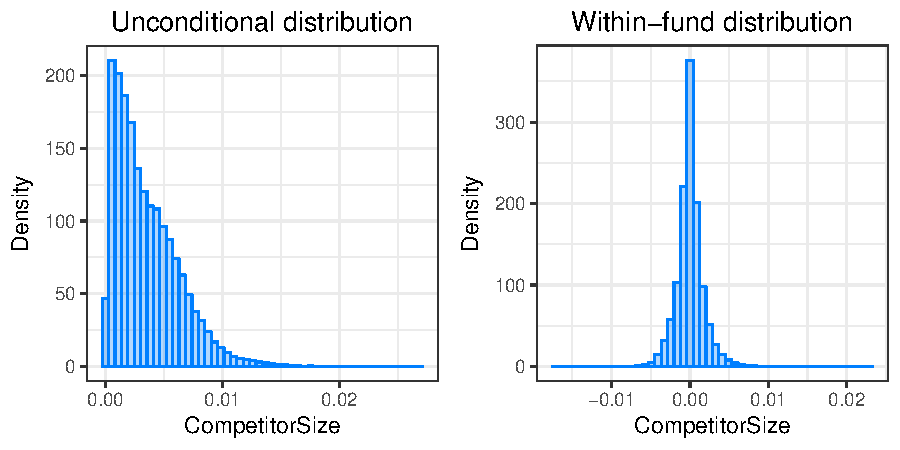
\includegraphics{04-data_files/figure-latex/histograms-1} 

}

\caption{Histograms of $CompetitorSize$. The left panel illustrates the variable's unconditional distribution. The right panel shows the distribution after demeaning fund-by-fund.}\label{fig:histograms}
\end{figure}

The time series of the cross-sectional average competitor size and
aggregate industry size are closely related (left panel of Figure
\ref{fig:industrySize}). The dynamics of fund similarity are
substantively different from those of aggregate industry size (right
panel of Figure \ref{fig:industrySize}). Average similarity displays a
negative trend in the first half of the sample. Similarity then
increases rapidly until August 2003, peaking a month before first news
of official investigations into the late trading scandal broke. Average
similarity shows renewed increases after 2006 until close to the end of
the sample.

\hypertarget{correlations}{%
\section{Correlations}\label{correlations}}

Panel A of Table \ref{tab:correlations} presents unconditional pairwise
correlations between variables, while Panel B presents within-fund
pairwise correlations. \(CompetitorSize\) is positively correlated with
\(IndustrySize\) both unconditionally (\(\rho=\) 0.38) and at the fund
level (\(\rho=\) 0.60). The residual within-fund variation in
\(CompetitorSize\) with respect to \(IndustrySize\) reflects
heterogenous dynamics in competitor size across funds pursuing different
investment strategies.\footnote{This residual variation is useful for
  identification, as the time series correlation between
  \(IndustrySize\) and a linear time trend is \$\rho=\$0.93, making
  industry level decreasing returns to scale hard to distinguish from
  simple trends in the data.}

There is a small but negative correlation between \(CompetitorSize\) and
risk adjusted gross returns, both unconditionally (\(\rho=\) -0.02) and
within-fund (\(\rho=\) -0.03). \(CompetitorSize\) tends to increase over
each fund's lifetime. The within-fund correlation between
\(CompetitorSize\) and \(FundAge\) is \(\rho=\) 0.51. The unconditional
correlation is markedly lower (\(\rho=\) 0.10), indicating that new
funds begin their operations exploiting relatively lightly contested
investment opportunities. \(CompetitorSize\) is highly correlated with
portfolio liquidity both unconditionally (\(\rho=\) 0.75) and
within-fund (0.63), evidence that more liquid market segments are
capable of absorbing higher levels of active investment. Consistent with
the joint determination of fund size, portfolio liquidity, turnover, and
expense ratios in \citet{pst17L}, larger funds tend to be more liquid,
trade less, and charge lower fees.

\hypertarget{sec:portfolio}{%
\chapter{Competition and Capital Allocation}\label{sec:portfolio}}

\hypertarget{decreasing-returns-to-competitor-scale}{%
\section{Decreasing Returns to Competitor
Scale}\label{decreasing-returns-to-competitor-scale}}

I develop empirical tests of hypotheses 1 and 2, using competitor scale
as the external constraint on the profitability of investment
opportunities. This choice is motivated by both the extant literature
and novel evidence from my sample. \citet{pst15} give time series
evidence that funds suffer from decreasing returns to aggregate industry
scale. In recent work, \citet{hkp17} provide cross-sectional evidence of
decreasing profitability due to inter-fund competition. I explore a
cross between the two approaches, by running within-fund tests of
decreasing returns to competitor scale. Appendix
\ref{sec:CSandPerformance} provides the details of my investigation. The
following is a brief summary of the results.

\begin{itemize}
\tightlist
\item
  A one standard deviation increase in competitor size is associated
  with a 78bp decrease in annual Fama-French three factor adjusted
  returns.
\item
  Competitor size subsumes the negative effect of aggregate industry
  size in a head to head horse race.
\item
  The negative impact of competitor size is smaller for funds which on
  average hold more liquid portfolios. This is consistent with liquidity
  constraints as the channel for decreasing returns to competitor scale.
\item
  The negative impact of competitor size is smaller when funds tilt
  toward more liquid portfolios. These results suggest that increased
  portfolio liquidity shelters funds from the pernicious effects of
  decreasing returns to scale.
\item
  Holding skill fixed, funds make more when they hold less liquid
  portfolios. One interpretation is that funds increase portfolio
  concentration when they perceive favorable investment opportunities in
  their core competence.
\end{itemize}

\hypertarget{empirical-strategy}{%
\section{Empirical Strategy}\label{empirical-strategy}}

Motivated by decreasing returns to competitor scale, I parametrize the
profitability of the fund's time \(t\) investment opportunities as
\begin{equation}
g(x_{i,t})=CompetitorSize_{i,t}^{-\gamma}. 
\label{eq:muParam}
\end{equation} This is a sensible choice in that the fund's alpha before
transaction costs is a decreasing function of competitor scale,
asymptoting to zero as the market approaches perfect competition.

The fraction of assets under active management in \citet{bg04} is
similar in spirit to active share (denoted \(AS\)) from \citet{cp09},
\citet{petajisto13}.\footnote{\citet{cremers17} shows that for funds
  that do not short or use leverage, active share is equal to one minus
  the sum of holdings that overlap with the benchmark. Letting \(J\) be
  the set of stocks held by the fund and \(B\) the set of stocks in the
  benchmark \(b\), we have
  \[ ActiveShare=1-\sum_{j\in J\cap B} \min\{ w_{i,j},w_{b,j} \}.\]} The
\citet{pst17L} portfolio choice maps directly into data on turnover and
fund holdings. Therefore, letting
\(y_{i,t}\in\{AS_{i,t},\left(TL^{-1/2}\right)_{i,t}\}\), the equilibrium
relation (with potential information asymmetry) in equation
\eqref{eq:csEQa} implies the regression model \begin{equation}
\ln(y_{i,t})=\alpha_t + \eta_1 \ln(FundSize_{i,t}) +\eta_2 \ln(f_{i,t}) + \gamma\ln(CompetitorSize_{i,t}) + \varepsilon_{i,t}.
\label{eq:regCS}
\end{equation} \(y\) and \(CompetitorSize\) are both calculated based on
the same portfolio weights. To ensure that my findings are not an
artifact of measurement, I consider quarter end holding reports only,
and calculate the log change in \(CompetitorSize\), holding constant
previous quarter-end similarity weights. That is, let \(t\) be quarter
end dates, and define \begin{equation}
\Delta CS_{i,t}=\ln \left(\sum_{j\neq i} \psi_{i,j,t-1} FundSize_{j,t}\right) - \ln \left(\sum_{j\neq i} \psi_{i,j,t-1} FundSize_{j,t-1}\right).
\end{equation} Note that the fund's change in capital allocation from
\(t-1\) to \(t\) has no mechanical effect on \(\Delta CS\), as it is
determined only by changes in other fund size, holding similarity fixed.

I then estimate equation \eqref{eq:regCS} in quarterly first differences
as \begin{equation}
\Delta\ln(y_{i,t})=\alpha_t + \eta_1 \Delta\ln(FundSize_{i,t}) +\eta_2 \Delta\ln(f_{i,t}) + \gamma\Delta CS_{i,t} + \Delta\varepsilon_{i,t}.
\label{eq:fdReg}
\end{equation} I double cluster standard errors by fund and date
\(\times\) portfolio group.\footnote{
Fund portfolios are grouped using k-means cluster analysis of raw portfolio weights. Each month, this process constructs $k=10$ archetypal portfolios (serving as cluster centers). These model portfolios are constructed and then funds are assigned to them such that the sum of squared differences between the weights of fund portfolios and their assigned model portfolio is minimized.
} Under the hypothesis of symmetrically informed outside investors,
\(\gamma=0\). Under the joint hypothesis of decreasing returns to
competitor scale and asymmetric information, \(\gamma<0\). I also
perform the analysis separating out portfolio liquidity and its
components. In these regressions, the joint hypothesis of decreasing
returns to competitor scale and asymmetric information implies
\(\gamma>0\).

\hypertarget{results}{%
\section{Results}\label{results}}

Table \ref{tab:fundResponse} presents results from empirical tests
evaluating hypothesis 1 against hypothesis 2. The statistically
significant coefficients on \(\Delta CS\) provide a rejection of the
hypothesis that managers and outside investors are symmetrically
informed of investment opportunities captured by changes in the scale of
competing funds.

The results are consistent with managers reacting optimally to
decreasing returns to own and competitor scale by scaling back active
management. A one percent increase in competitor size is associated with
a -0.05bp change in active share, and a -0.47bp change in the turnover
to portfolio liquidity ratio. Increases in competitor scale are
associated with statistically significant increases in each component of
portfolio liquidity. A one percent increase in own size is associated
with a -0.02bp change in active share, and a -0.18bp change in turnover
to portfolio liquidity.

\label{tab:fundResponse}Capital Allocation and Competitor Size Observations
are first differences at the fund \(\times\) quarter level, from
1980-2016. Dependent variables are noted in the column headers. \(AS\)
is active share relative to self-declared benchmarks {[}\citet{cp09};
petajisto13{]}, covering years 1980-2009. \(TL^{-1/2}\) is the turnover
to portfolio liquidity ratio, as in \citet{pst17L}. \(S\), \(D\), \(C\),
and \(B\) are the components of portfolio liquidity, namely stock
liquidity, diversification, coverage, and balance (each calculated with
respect to all U.S. equity).
\(\Delta CS_{i,t}=\ln\left(\sum_{j\neq i} \psi_{i,j,t-1} FundSize_{j,t} \right) - \ln\left(\sum_{j\neq i} \psi_{i,j,t-1} FundSize_{j,t-1}\right)\)
is the change in log competitor size, holding previous quarter end
similarity weights fixed. Standard errors are double clustered by fund
and portfolio group \(\times\) quarter, and reported in parentheses.
Asterisks denote statistical significance: \(\ast\ast\ast\) p\$

Dep. Var.:

\(\Delta\ln(AS)\)

\(\Delta\ln(TL^{-1/2})\)

\(\Delta\ln(L)\)

\(\Delta\ln(S)\)

\(\Delta\ln(D)\)

\(\Delta\ln(C)\)

\(\Delta\ln(B)\)

\(\Delta CS\)

-0.051***

-0.472***

0.788***

0.659***

0.533***

0.173***

0.435***

(0.020)

(0.064)

(0.083)

(0.088)

(0.061)

(0.035)

(0.052)

\(\Delta\ln(FundSize)\)

-0.016***

-0.184***

0.218***

0.108***

0.196***

0.115***

0.115***

(0.003)

(0.016)

(0.018)

(0.013)

(0.016)

(0.012)

(0.011)

\(\Delta\ln(f)\)

-0.018

0.063

-0.009

-0.025

0.005

0.023

-0.015

(0.014)

(0.041)

(0.032)

(0.026)

(0.031)

(0.024)

(0.026)

\(\Delta \ln(T)\)

-0.013*

-0.006

-0.011*

0.001

-0.014***

(0.007)

(0.005)

(0.006)

(0.004)

(0.005)

\(\Delta\ln(D)\)

-0.340***

(0.018)

\(\Delta\ln(S)\)

-0.570***

-0.194***

-0.458***

(0.017)

(0.013)

(0.021)

\(\Delta\ln(B)\)

-0.114***

(0.011)

\(\Delta\ln(C)\)

-0.229***

(0.021)

Fixed Effects

\(\bullet\) Quarter

Yes

Yes

Yes

Yes

Yes

Yes

Yes

Observations

34,984

57,146

57,146

57,146

57,146

57,146

57,146

\(R^2\)

0.025

0.028

0.059

0.218

0.224

0.101

0.180

\(R^2\) (proj. model)

0.005

0.018

0.045

0.202

0.209

0.081

0.171

\citet{pst17L} argue that unit trading costs might vary by fund segment,
implying a model with segment \(\times\) time fixed effects. To
accommodate segment level variation in trading costs, I redo the
analysis with benchmark \(\times\) quarter fixed effects in
Table\textasciitilde{}\{tab:fundResponseMXBim\}. The results remain
similar.

Overall, my findings are consistent with fund managers reacting
optimally to short-term changes in investment opportunities that are not
immediately apparent to outside investors. This interpretation fits in
with a growing literature on the adjustments managers make in response
to time variations in the investment opportunity set. \citet{knv16} show
that managers are better at timing factors during recessions when the
covariance between asset returns is high. \citet{pst17} provide evidence
that funds increase trading when faced with more favorable
opportunities.

\hypertarget{sec:scandal}{%
\chapter{Evidence From the 2003 Mutual Fund Scandal}\label{sec:scandal}}

In September 2003, the New York Attorney General's office launched
investigations into several high-profile mutual fund families for
illegal trading practices. Families were charged with allowing favored
clients to trade fund shares at stale prices at the expense of ordinary
shareholders \citep{hw05, zitzewitz06}. By the end of October 2004,
official investigations had been announced against a total of
twenty-five mutual fund families.

\citet{hw05} and \citet{mccabe08} argue that investors penalized tainted
funds with large outflows. This is borne out in my data. Figure
\ref{fig:scandalFlows} plots mean net flows by scandal
involvement.\footnote{I follow Table 1 of \citet{hw05} for classifying
  fund families embroiled in the scandal. The following is the list of
  fund families tainted by the scandal by month of the news date of
  investigation. September 2003: Alliance Bernstein, Franklin Templeton,
  Gabelli, Janus, Nations, One Group, Putnam, Strong. October 2003:
  Alger, Federated. November 2003: Excelsior/US Trust, Fremont, Loomis
  Sayles, PBHG. December 2003: AIM/Invesco, MFS, Heartland. January
  2004: Columbia, Scudder, Seligman. February 2004: PIMCO. March 2004:
  ING, RS. August 2004: Evergreen. October 2004: Sentinel.\\
  I identify funds belonging to these families as of August 2003 in my
  sample based on the share class names in the CRSP mutual fund dataset.
  I classify 289 of the 1,462 funds in my sample in August 2003 with
  existing holdings and gross returns as members of future tainted
  families. Table\textasciitilde{}\ref{tab:snapShot200308} presents a
  snapshot of summary statistics as of August 2003 by future scandal
  involvement. Scandal funds are slightly older, larger, and have higher
  turnover to portfolio liquidity and expense ratios.}

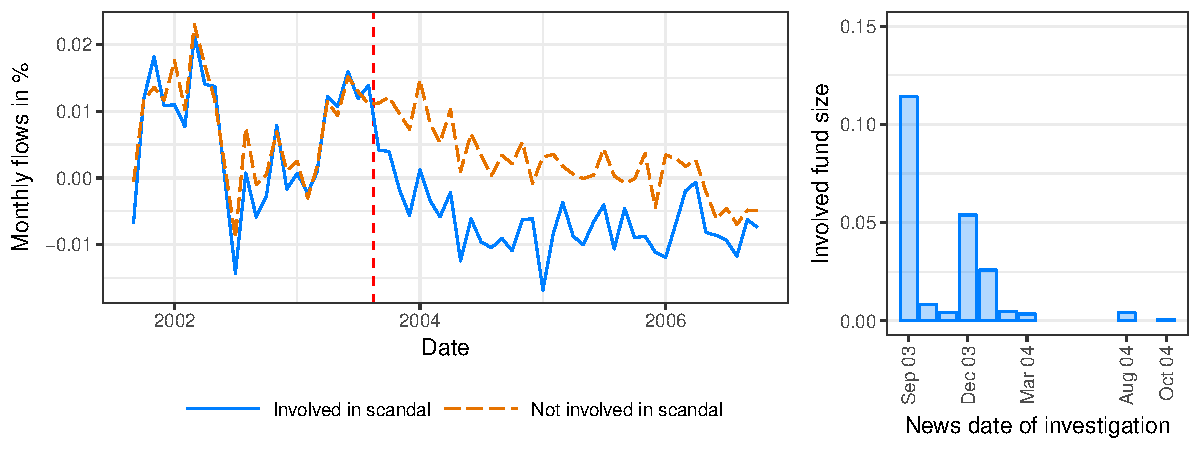
\includegraphics{06-scandal_files/figure-latex/scandalFlows-1.pdf}

The two series track each other closely in the two years prior to the
scandal, and diverge abruptly in September 2003. The wedge between the
two groups persists until the end of 2006, coincident with the final
settlements negotiated with the Securities and Exchange Commission
\citep{zitzewitz09}.\footnote{The difference is statistically
  significant. I estimate a regression using a two year pre- and
  post-scandal window of observations of the form \[
  flow_{i,t}=\alpha_i + \alpha_t + \gamma Post_{i,t} +\varepsilon_{i,t},
  \] where \(Post_{i,t}\) is an indicator for post news date for scandal
  funds. I find \(\gamma=-9.16\)\% per year, with t-statistic of
  \(4.6\).}

I conclude that the scandal caused a significant reallocation of
resources away from tainted funds. Unless flows are perfectly
offsetting, this shift will cause a relative reduction in the competitor
size of the most similar funds. Under decreasing returns to competitor
scale, we would expect the investment opportunities of these funds to
improve in relative terms, leading them to differentially expand active
management and earn higher returns.

I test these hypotheses by comparing untainted funds with differential
pre-scandal similarity to prospective scandal funds. I discard tainted
funds as the internal upheaval following the scandal likely had a direct
impact on their performance and investment behavior.\footnote{In the
  aftermath of the investigations, several executives stepped down, and
  a number of portfolio managers were fired. Perhaps the highest profile
  casualty of the scandal was Richard S. Strong, founder of Strong
  Capital Management, who resigned in December 2003. Strong would go on
  to pay \$60 million in settlements and be barred from the industry.
  Strong Capital itself was acquired by Wells Fargo in 2004.} I take two
approaches. The first is a straightforward
difference-in-differences-style comparison of fund outcomes before and
after the scandal as a function of their pre-scandal exposure to tainted
funds. The second approach links fund outcomes directly to variation in
competitor size attributable to abnormal flows among tainted funds. I
first present the analysis on fund capital allocation, followed up by
the analysis of fund performance.

\hypertarget{sec:scandalID}{%
\section{Before and After Analysis}\label{sec:scandalID}}

I relate fund-by-fund differences in pre-scandal \([2003m8-W\),
\(2003m8]\) and post-scandal \([2004m11\), \$2004m11+W{]} \$ outcomes to
pre-scandal exposure to competition from tainted funds. I consider
\(W\in\{1,2\}\) year windows. For a fund to be included in the
estimation sample, it must have available holdings information for
August 2003, and I must observe it both in the pre- and the post-scandal
period.

I measure pre-scandal exposure as the proportion of competitor size
attributable to prospective tainted funds as of August 2003. Let
\(\Phi\) denote the set of funds that belong to families later
investigated, and define \begin{equation}
ScandalExposure_i = \frac{\sum_{j\in \Phi} \psi_{i,j,2003m8} FundSize_{j,2003m8}}{\sum_{j\neq i}\psi_{i,j,2003m8} FundSize_{j,2003m8}}.
\end{equation} On average, \(22\)\% of untainted funds' competitor size
is due to tainted fund families. Exposure ranges from 7\% to over 40\%,
with upper quartile 25\% and lower quartile 19\%.

To present interpretable summary statistics, I sort funds into high and
low exposure groups depending on whether their \(ScandalExposure\) is
above or below the cross-sectional median.
Table\textasciitilde{}\ref{tab:snapShotHL200308} gives a snapshot taken
in August 2003. High exposure funds are slightly smaller, have higher
turnover to portfolio liquidity ratios, expense ratios,
\(CompetitorSize\), and worse performance. Fund age is almost identical
across the two groups, limiting the plausibility of life cycle effects
as an explanation for differences in outcome paths.

Figure \ref{fig:exposureDID} summarizes the identifying variation in the
data. I plot the groupwise cross-sectional mean of within-fund
deviations for competitor size, log active share, and log turnover to
portfolio liquidity ratio. The differential impact of the scandal across
groups is identified by the difference in the pre- and post-scandal
period wedges between the series. The \(CompetitorSize\) of the low
exposure group overall trends upward, despite a small dip in the middle
of the scandal period. The \(CompetitorSize\) of high exposure funds
drops more substantively during the scandal, and remains flat for almost
a year after the end of the scandal period. The historical accident of
scandal-related outflows at involved funds appear to have insulated
their closest competitors from contemporaneous increases in the
aggregate size of the industry.

\begin{figure}
\centering
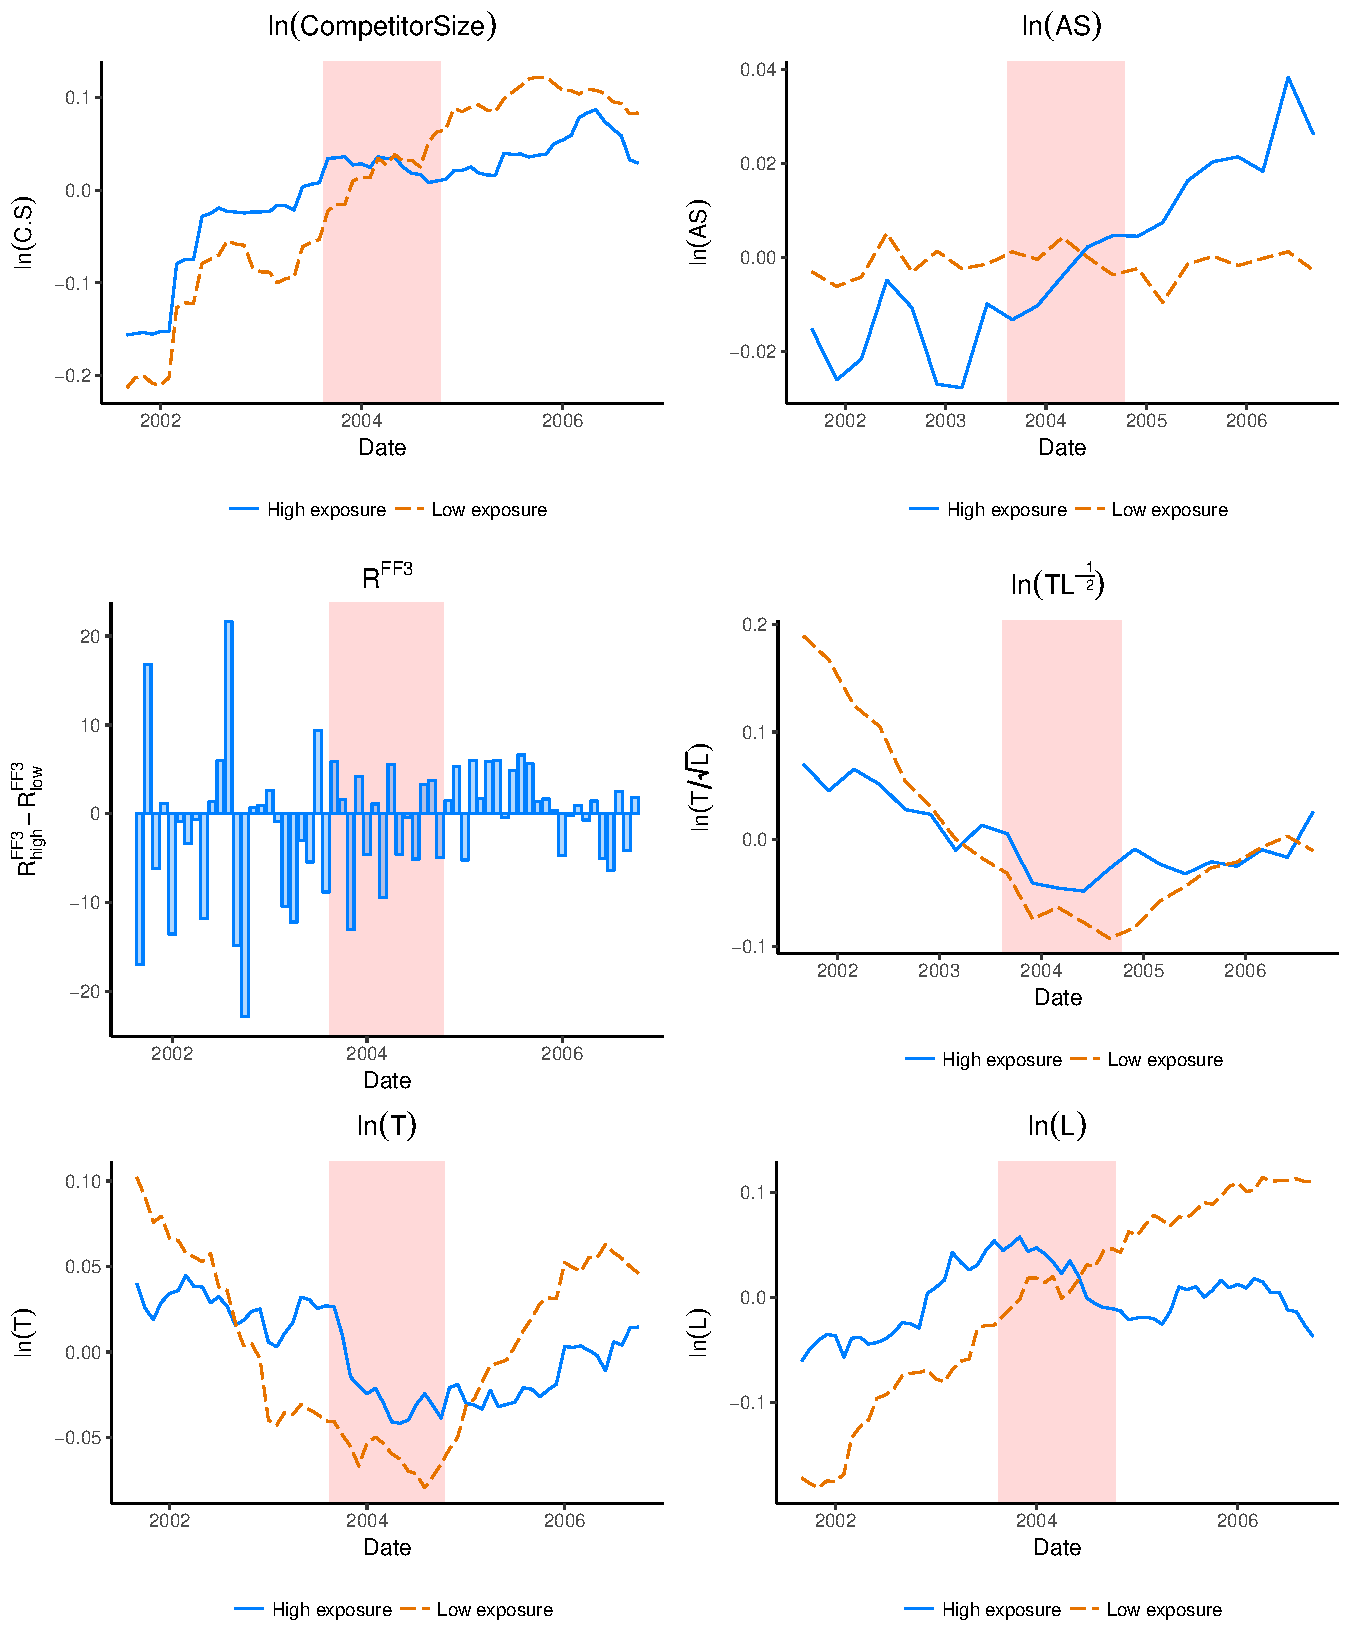
\includegraphics{06-scandal_files/figure-latex/exposureDID-1.pdf}
\caption{\label{fig:exposureDID}Untainted fund outcomes by exposure to
competition from scandal funds. Funds are sorted into high and low
exposure groups depending on whether their \(ScandalExposure\) is above
or below the cross-sectional median. The \(\ln(CompetitorSize)\),
\(\ln(AS)\), and \(\ln(TL^{-1/2})\) panels plot cross-sectional means of
the variables' deviations from their respective within fund means across
exposure groups. The \(R^{FF3}\) panel plots the difference between the
cross-sectional means of the within fund deviations of three factor
adjusted gross returns across the two groups. Vertical lines correspond
to August 2003, the month before the announcement of the first
investigations, and October 2004, the month of the last investigations
according to Table 1 of \citet{hw05}.}
\end{figure}

The turnover to portfolio liquidity ratio of the low exposure group
exhibits a steady decline until late 2005, despite a momentary increase
during the scandal. The high exposure group shows parallel trends until
the beginning of the scandal period. Consistent with improved investment
opportunities during the scandal, high exposure funds substantially
decreased portfolio liquidity and increased turnover during 2004. The
gap in within-fund turnover to portfolio liquidity ratios only begins to
close at the end of 2006 as abnormal flows at scandal funds vanish.
Active share of low exposure funds is essentially flat during this
period, whereas active share of high exposure funds show steady
increases during and after the scandal.

Given the volatility of returns, for easier comparison of fund
performance I plot the difference between high and low exposure group
cross-sectional means of within-fund three factor adjusted returns. High
exposure funds relatively underperform low exposure funds in the
pre-scandal period, are essentially even during the scandal, and enjoy a
string of relative outperformance in the year after the end of the
scandal period. The differential relative before and after performance
of the two groups is consistent with decreasing returns to competitor
scale.

To formally test for differential differences in before and after
outcomes as a function of ex ante exposure to competition from
prospective scandal funds, I perform regressions of the form
\begin{equation}
y_{i,t} = \alpha_i + \alpha_t + \gamma \left( \mathbb{I}_t \times ScandalExposure_i \right) + \mathbf{X}_{i,t}\Gamma + \varepsilon_{i,t},
\label{eq:didReg}
\end{equation} where \(\mathbf{X}_{i,t}\) includes log fund size and
expense ratio, as dictated by theory. In the regression, exposure is a
continuous variable.\footnote{
Unreported binned scatter plots suggest reasonably linear relations between $ScandalExposure$ and outcome variables after residualizing by fund and time fixed effects.
} I double cluster standard errors by fund and portfolio group
\(\times\) time. I normalize \(ScandalExposure\) by its interquartile
range (\(\approx 6\)\%).

\label{tab:scandalSpillover}Capital Allocation and the Scandal: Before and
After Analysis Dependent variables are identified in the column headers.
\(\ln(C.S.)\) is an abbreviation for \(\ln(CompetitorSize)\). For
regressions with \(\ln(TL^{-1/2})\) as the dependent variable,
observations are at the fund-month level. Other specifications are at
the fund-report date level. The estimation sample includes only funds
not directly involved in the scandal. It covers the period
\(\{(2003m8-W, 2003m8], [2004m11, 2004m11 + W) \}\), where \(W\)
corresponds to the number of years specified. \(ScandalExposure\)
(abbreviated to \(ScanEx\)) is the fraction of untainted funds'
\(CompetitorSize\) due to portfolio similarity with future scandal funds
in August 2003 (see Section \ref{sec:scandalID} for details). I
normalize \(ScandalExposure\) by its interquartile range. \(\mathbb{I}\)
is an indicator for the post scandal period. Standard errors are double
clustered by fund and portfolio group \(\times\) quarter, and reported
in parentheses. Asterisks denote statistical significance:
\(\ast\ast\ast\) p\$

Dep. Var.:

\(\ln(C.S.)\)

\(\ln(AS)\)

\(\ln(TL^{-1/2})\)

\(\ln(L)\)

\(\ln(S)\)

\(\ln(D)\)

\(\ln(C)\)

\(\ln(B)\)

1 year window

\(\mathbb{I}\times ScanEx\)

-0.034*

0.029***

0.010

-0.100***

-0.105***

-0.039*

-0.032**

-0.011

(0.020)

(0.006)

(0.031)

(0.025)

(0.019)

(0.022)

(0.015)

(0.016)

\(\ln(FundSize)\)

0.149***

-0.018***

-0.205***

0.184***

0.088***

0.148***

0.074***

0.084***

(0.017)

(0.006)

(0.025)

(0.022)

(0.013)

(0.021)

(0.016)

(0.015)

\(\ln(f)\)

-0.097

0.004

0.113

-0.073

-0.169**

0.040

0.105

-0.061

(0.073)

(0.027)

(0.117)

(0.108)

(0.076)

(0.091)

(0.072)

(0.071)

\(\ln(T)\)

-0.063***

-0.065***

-0.025

0.023

-0.049***

(0.024)

(0.014)

(0.022)

(0.014)

(0.015)

\(\ln(D)\)

-0.216***

(0.022)

\(\ln(S)\)

-0.425***

-0.218***

-0.236***

(0.036)

(0.033)

(0.039)

\(\ln(B)\)

-0.056**

(0.025)

\(\ln(C)\)

-0.077**

(0.034)

Fixed Effects

\(\bullet\) Fund

Yes

Yes

Yes

Yes

Yes

Yes

Yes

Yes

\(\bullet\) Time

Yes

Yes

Yes

Yes

Yes

Yes

Yes

Yes

Observations

13,666

11,773

46,660

13,291

13,291

13,291

13,291

13,291

\(R^2\)

0.895

0.878

0.860

0.943

0.980

0.914

0.914

0.848

\(R^2\) (proj. model)

0.065

0.027

0.043

0.083

0.154

0.114

0.071

0.063

2 year window

\(\mathbb{I}\times ScanEx\)

-0.034*

0.029***

0.010

-0.100***

-0.105***

-0.039*

-0.032**

-0.011

(0.020)

(0.006)

(0.031)

(0.025)

(0.019)

(0.022)

(0.015)

(0.016)

\(\ln(FundSize)\)

0.149***

-0.018***

-0.205***

0.184***

0.088***

0.148***

0.074***

0.084***

(0.017)

(0.006)

(0.025)

(0.022)

(0.013)

(0.021)

(0.016)

(0.015)

\(\ln(f)\)

-0.097

0.004

0.113

-0.073

-0.169**

0.040

0.105

-0.061

(0.073)

(0.027)

(0.117)

(0.108)

(0.076)

(0.091)

(0.072)

(0.071)

\(\ln(T)\)

-0.063***

-0.065***

-0.025

0.023

-0.049***

(0.024)

(0.014)

(0.022)

(0.014)

(0.015)

\(\ln(D)\)

-0.216***

(0.022)

\(\ln(S)\)

-0.425***

-0.218***

-0.236***

(0.036)

(0.033)

(0.039)

\(\ln(B)\)

-0.056**

(0.025)

\(\ln(C)\)

-0.077**

(0.034)

Fixed Effects

\(\bullet\) Fund

Yes

Yes

Yes

Yes

Yes

Yes

Yes

Yes

\(\bullet\) Time

Yes

Yes

Yes

Yes

Yes

Yes

Yes

Yes

Observations

13,666

11,773

46,660

13,291

13,291

13,291

13,291

13,291

\(R^2\)

0.895

0.878

0.860

0.943

0.980

0.914

0.914

0.848

\(R^2\) (proj. model)

0.065

0.027

0.043

0.083

0.154

0.114

0.071

0.063

Table \ref{tab:scandalSpillover} presents results. The one (two) year
window estimate implies a \(6.7\)\% (\(3.5\)\%) post-scandal reduction
in \(CompetitorSize\) for untainted funds at the 75\(^{\text{th}}\)
percentile of \(ScandalExposure\) relative to untainted funds at the
25\(^{\text{th}}\) percentile of \(ScandalExposure\). The same
difference in \(ScandalExposure\) is associated with a \(2.4\)\%
(\(2.6\)\%) relative increase in active share, and a \(6.3\)\%
(\(4.4\)\%) increase in the turnover to portfolio liquidity ratio. The
coefficients also imply a relative decline in portfolio liquidity and
its components for high exposure funds. These findings are consistent
with high exposure funds increasing activeness in response to softened
competition.

The main concern with identification based on comparing pre- and
post-event periods across groups is that the measured effect might be
the manifestation of favorable trends across the groups in the
pre-period. I test for differential trends in the pre-period as a
function of \(ScandalExposure\) by estimating the regression
\begin{equation}
y_{i,t} = \alpha_i + \alpha_t + \gamma \left(t \times ScandalExposure_i\right) + \mathbf{X}_{i,t}\Gamma + \varepsilon_{i,t},
\end{equation} where \(t\) is a linear time trend and
\(\mathbf{X}_{i,t}\) includes the usual controls. I estimate this
regression on pre-period observations. Differential pre-trends by
\(ScandalExposure\) would be a concern if the coefficient on the trend
interaction was statistically significant and of the same sign as the
corresponding interaction coefficient in Table
\ref{tab:scandalSpillover}. Results from these specifications fail to
reject the null hypothesis of no differential trends in the pre-period
(Table\textasciitilde{}\ref{tab:scandalSpilloverPreTrend}).

\hypertarget{sec:linkFlows}{%
\section{\texorpdfstring{Linking \(CompetitorSize\) Directly to Abnormal
Flows}{Linking CompetitorSize Directly to Abnormal Flows}}\label{sec:linkFlows}}

The analysis above does not explicitly model fund outcomes as a function
of scandal flows. In this section, I explore a more sophisticated
approach. I first estimate outflows at tainted funds attributable to the
scandal. In turn, I relate untainted fund outcomes to variation in
competitor size explained by abnormal tainted competitor outflows.

I use a linear model to decompose variation in fund flows between the
effects of the scandal and baseline variation. I pool tainted and
untainted funds in the two year window surrounding the scandal period,
consisting of observations from September 2001 to October 2006. Consider
scandal funds as being from the same cohort \(d\) if news of
investigation into their trading practices broke in month \(d\). Denote
the cohort of fund \(j\) as \(j^{(d)}\). Let
\(\mathbb{I}_{t\geq j^{(d)}}\) be an indicator for post investigation
months for fund \(j\), and define \(\mathbb{I}_{d,t}\) as cohort
\(\times\) time dummy variables. I regress flows on the full set of
post-investigation cohort \(\times\) time indicators, controlling for
fund and time fixed effects: \begin{equation}
flow_{j,t}=\alpha_j+\alpha_t +\beta_{j^{(d)},t} \left( \mathbb{I}_{t\geq j^{(d)}}\mathbb{I}_{j^{(d)},t} \right) + \varepsilon_{j,t}.
\label{eq:cohortReg}
\end{equation} I interpret the betas as the path of abnormal flows
attributable to the scandal for each cohort. I cumulate abnormal flows
at each post-scandal date as \begin{equation}
\hat{f}_{j,t} = \prod_{\tau\geq j^{(d)}}^t \left(1+\hat{\beta}_{j^{(d)},t}\right) - 1.
\end{equation} I construct \(ScandalOutFlow\) for untainted fund \(i\)
as the similarity- and size-weighted cumulative abnormal negative net
flow among tainted funds \(j\in\Phi\): \begin{equation}
ScandalOutFlow_{i,t}= -\sum_{j\in \Phi} \psi_{i,j,2003m8} \left(\hat{f}_{j,t} FundSize_{j,2003m8} \right).
\label{eq:scandalOutFlow}
\end{equation}

Figure \ref{fig:scandalOutFlow} plots time series characteristics of
abnormal flows and \(ScandalOutFlow\). Abnormal flows are most negative
in the immediate aftermath of the announcement of the first
investigations, and gradually converge to zero near the end of 2006.
This pattern maps into almost linearly increasing cumulative outflows in
the first two years after the scandal, reflected in the observed pattern
in \(ScandaOutFlow\). Importantly for identifying differential spillover
effects of the scandal, total predicted outflows at competing tainted
funds vary substantially in the cross-section.

\begin{figure}
\centering
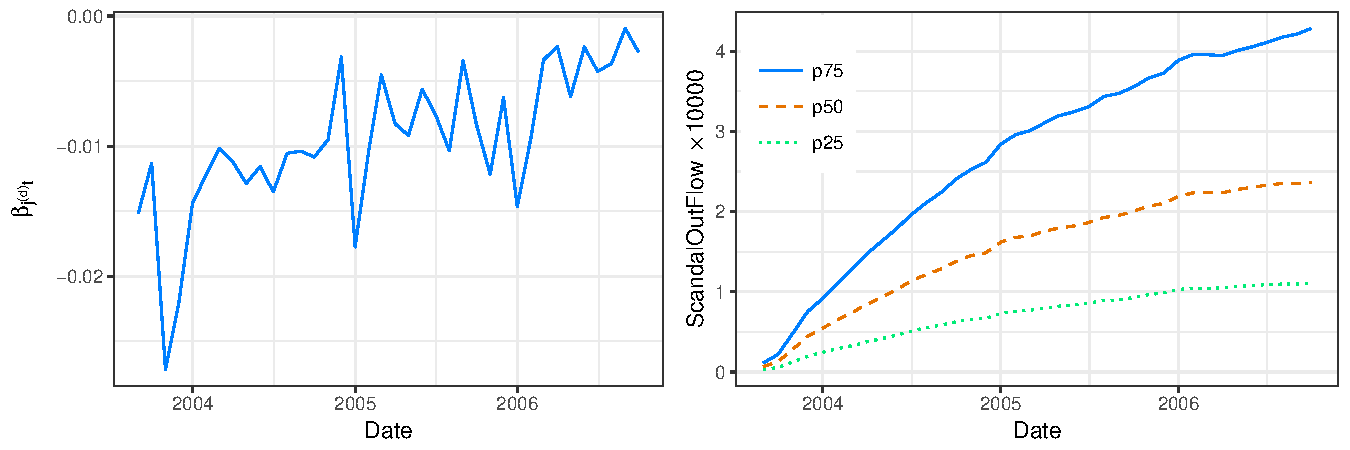
\includegraphics{06-scandal_files/figure-latex/scandalOutFlow-1.pdf}
\caption{\label{fig:scandalOutFlow}Abnormal flows and \(ScandalOutFlow\).
The left panel shows the cross-sectional mean coefficient on
post-scandal cohort \(\times\) time fixed effects from Equation
\eqref{eq:cohortReg}. The right panel shows the time series of
cross-sectional percentiles of \(ScandalOutFlow\) across untainted
funds, calculated according to Equation \eqref{eq:scandalOutFlow}.}
\end{figure}

I link tainted funds' flows directly to untainted fund outcomes through
the reduced form regressions \begin{equation}
    y_{i,t}=\alpha_i+\alpha_t+\gamma ScandalOutFlow_{i,t} + \mathbf{X}_{i,t}\Gamma + \varepsilon_{i,t},
\end{equation} where \(\mathbf{X}_{i,t}\) includes log size and expense
ratio. Table \ref{tab:scandalSpilloverIV} presents results. The
coefficient on \(ScandalOutFlow\) represents the expected difference in
outcomes between funds across the variable's interquartile range. Moving
from the 25\(^{\text{th}}\) to the 75\(^{\text{th}}\) percentile of
abnormal scandal-affected competitor outflow is associated with an
approximately \(18\)\% relative decline in competitor size. Consistent
with the difference-in-differences-style analysis, the results indicate
that funds whose competitors were particularly affected by
scandal-related outflows expanded active management relative to funds
with less affected competitors, increasing active share, turnover to
portfolio liquidity ratios, and decreasing portfolio liquidity.

\label{tab:scandalSpilloverIV} Dependent variables are identified in the
column headers. For regressions with
\(\ln\left(TL^{-\frac{1}{2}}\right)\) as the dependent variable,
observations are at the fund-month level. Other specifications are at
the fund-report date level. The estimation sample includes untainted
funds during \(\{[2003m9-W, 2004m10+W] \}\), where \(W\) corresponds to
the number of years specified at the bottom of each panel.
\(ScandalOutFlow\) is the similarity-weighted cumulative abnormal
outflows attributable to the scandal among involved funds.
\(ScandalOutFlow\) is normalized by its interquartile range. See Section
\ref{sec:linkFlows} for details on the variable's construction.
\(\ln(C.S.)\) is an abbreviation for \(\ln(CompetitorSize)\). Standard
errors are double clustered by fund and portfolio group \(\times\)
quarter, and reported in parentheses. Asterisks denote statistical
significance: \(\ast\ast\ast\) p\$

Dep. Var.:

\(\ln(C.S.)\)

\(\ln(AS)\)

\(\ln(TL^{-1/2})\)

\(\ln(L)\)

\(\ln(S)\)

\(\ln(D)\)

\(\ln(C)\)

\(\ln(B)\)

1 year window

\(ScandalOutFlow\)

-0.181***

0.059***

0.114***

-0.221***

-0.120***

-0.181***

-0.076***

-0.127***

(0.016)

(0.007)

(0.024)

(0.023)

(0.015)

(0.021)

(0.015)

(0.014)

\(\ln(FundSize)\)

0.092***

-0.010*

-0.149***

0.143***

0.080***

0.116***

0.075***

0.056***

(0.017)

(0.005)

(0.027)

(0.022)

(0.013)

(0.021)

(0.016)

(0.015)

\(\ln(f)\)

-0.066

-0.009

0.036

-0.027

-0.062

0.009

0.078

-0.064

(0.070)

(0.024)

(0.111)

(0.089)

(0.062)

(0.083)

(0.062)

(0.060)

\(\ln(T)\)

-0.057***

-0.045***

-0.038**

0.011

-0.052***

(0.019)

(0.011)

(0.018)

(0.011)

(0.015)

\(\ln(D)\)

-0.267***

(0.024)

\(\ln(S)\)

-0.522***

-0.269***

-0.318***

(0.045)

(0.035)

(0.047)

\(\ln(B)\)

-0.097***

(0.029)

\(\ln(C)\)

-0.155***

(0.043)

Fixed Effects

\(\bullet\) Fund

Yes

Yes

Yes

Yes

Yes

Yes

Yes

Yes

\(\bullet\) Time

Yes

Yes

Yes

Yes

Yes

Yes

Yes

Yes

Observations

12,095

10,334

39,784

11,689

11,689

11,689

11,689

11,689

\(R^2\)

0.935

0.933

0.904

0.967

0.988

0.949

0.950

0.901

\(R^2\) (proj. model)

0.088

0.073

0.027

0.107

0.172

0.174

0.107

0.103

2 year window

\(ScandalOutFlow\)

-0.168***

0.061***

0.110***

-0.209***

-0.125***

-0.162***

-0.075***

-0.104***

(0.015)

(0.007)

(0.022)

(0.020)

(0.014)

(0.019)

(0.015)

(0.013)

\(\ln(FundSize)\)

0.113***

-0.012**

-0.182***

0.156***

0.083***

0.128***

0.072***

0.070***

(0.014)

(0.005)

(0.023)

(0.019)

(0.012)

(0.018)

(0.015)

(0.013)

\(\ln(f)\)

-0.132**

0.011

0.135

-0.110

-0.169**

-0.016

0.076

-0.090

(0.059)

(0.023)

(0.098)

(0.096)

(0.070)

(0.080)

(0.061)

(0.063)

\(\ln(T)\)

-0.049**

-0.049***

-0.024

0.017

-0.043***

(0.019)

(0.011)

(0.018)

(0.012)

(0.013)

\(\ln(D)\)

-0.259***

(0.020)

\(\ln(S)\)

-0.506***

-0.254***

-0.305***

(0.035)

(0.031)

(0.038)

\(\ln(B)\)

-0.088***

(0.023)

\(\ln(C)\)

-0.127***

(0.032)

Fixed Effects

\(\bullet\) Fund

Yes

Yes

Yes

Yes

Yes

Yes

Yes

Yes

\(\bullet\) Time

Yes

Yes

Yes

Yes

Yes

Yes

Yes

Yes

Observations

18,904

16,211

63,055

18,309

18,309

18,309

18,309

18,309

\(R^2\)

0.907

0.898

0.869

0.951

0.982

0.924

0.922

0.860

\(R^2\) (proj. model)

0.103

0.086

0.046

0.117

0.181

0.164

0.095

0.096

In additional analyses I isolate the variation in \(CompetitorSize\)
attributable to abnormal flows at tainted competitors, and measure its
impact on capital allocation. I perform two-stage least squares (2SLS)
regressions, instrumenting for \(\ln(CompetitorSize)\) by
\(ScandalOutFlow\) in the specification \begin{equation}
    y_{i,t}=\alpha_i+\alpha_t + \gamma \ln(CompetitorSize_{i,t}) + \mathbf{X}_{i,t}\Gamma+\varepsilon_{i,t},
\end{equation} where \(y_{i,t}\) is log active share or log
turnover-liquidity ratio, and \(\mathbf{X}\) the usual controls.
Table\textasciitilde{}\ref{tab:scandal2SLS} presents results. As
expected based on the first column of Table
\ref{tab:scandalSpilloverIV}, the first stage F-statistics are high, and
\(ScandalOutFlow\) passes the relevance criterion. Consistent with
earlier results, variation in competitor size attributable to
\(ScandalOutFlow\) is associated with decreased active management and
increased portfolio liquidity.

\subsection{Controlling for Sector Level Shocks}

As an additional robustness check to ensure my results are not an
artifact of common sector level shocks, I re-estimate the analysis using
benchmark \(\times\) time fixed effects. The results remain similar
(Tables\textsubscript{\ref{tab:scandalSpilloverMXBim},}\ref{tab:scandalSpilloverPreTrendMXBim},\textsubscript{\ref{tab:scandalSpilloverIVMXBim},}\ref{tab:scandal2SLSmXbim}).

\subsection{Fund Performance}

The analysis presented so far is consistent with competitors of
scandal-tainted funds reacting to improved investment opportunities by
increasing capital allocated to active strategies. According to this
line of reasoning we would expect the same funds to experience
relatively improved performance. To investigate, in Table
\ref{tab:scandalPerformance} I perform analyses similar to those
presented above, but with risk adjusted gross returns as the outcome
variable of interest. The results demonstrate that close competitors of
tainted funds indeed saw an increase in relative performance following
the scandal.

\label{tab:scandalPerformance}Fund Performance and the Scandal The dependent
variable is Fama-French 3 factor adjusted gross returns, in annual
percent units. Observations are monthly. The estimation sample includes
only funds not tainted by the scandal. In columns (1)-(4) regressions
are estimated by ordinary least squares. In columns (5)-(6), regressions
are estimated by two stage least squares, instrumenting
\(\ln(CompetitorSize)\) with \(ScandalOutFlow\). In columns (1)-(2), the
sample includes \(\{(2003m8-W, 2003m8], [2004m11,2004m11+W) \}\), where
\(W\) corresponds to the number of years specified. In columns (3)-(6),
the sample is taken over the period \(\{[2003m9-W, 2004m10+W] \}\).
\(ScandalExposure\) (abbreviated to \(ScanEx\)) is the fraction of
untainted funds' \(CompetitorSize\) due to portfolio similarity with
future scandal funds in August 2003 (see Section \ref{sec:scandalID} for
details). I normalize \(ScandalExposure\) by its interquartile range.
\(\mathbb{I}\) is an indicator for the post scandal period.
\(ScandalOutFlow\) is the similarity-weighted cumulative abnormal
outflows attributable to the scandal among involved funds.
\(ScandalOutFlow\) is normalized by its interquartile range. See Section
\ref{sec:linkFlows} for details on the variable's construction.
Benchmarks are the indexes which yield the lowest active share, taken
from \citet{petajisto13}. Standard errors are double clustered by fund
and portfolio group \$ imes\$ month in columns (1)-(4), and by fund and
benchmark \(\times\) month in columns (5)-(6). Standard errors are
reported in parentheses. Asterisks denote statistical significance:
\(\ast\ast\ast\) p\$

\left(1\right)

\left(2\right)

\left(3\right)

\left(4\right)

\left(5\right)

\left(6\right)

1 year window

\(\mathbb{I}\times ScanEx\)

5.715***

3.944***

(1.130)

(0.770)

\(ScandalOutFlow\)

1.687**

2.237***

(0.829)

(0.674)

\(\ln(CompetitorSize)\)

-9.574**

-12.269***

(4.667)

(3.756)

\(\ln(FundSize)\)

-3.131***

-3.245***

-4.712***

-4.507***

-3.815***

-3.433***

(0.677)

(0.578)

(0.666)

(0.534)

(0.744)

(0.581)

Fixed Effects

\(\bullet\) Fund

Yes

Yes

Yes

Yes

Yes

Yes

\(\bullet\) Month

Yes

No

Yes

No

Yes

No

\(\bullet\) Benchmark \(\times\) Month

No

Yes

No

Yes

No

Yes

Observations

24,909

24,909

41,333

41,333

41,333

41,333

\(R^2\)

0.111

0.201

0.101

0.196

0.091

0.179

\(R^2\) (proj. model)

0.019

0.011

0.008

0.008

-0.003

-0.013

2 year window

\(\mathbb{I}\times ScanEx\)

2.509***

1.716***

(0.861)

(0.635)

\(ScandalOutFlow\)

0.405

0.843**

(0.491)

(0.361)

\(\ln(CompetitorSize)\)

-2.489

-5.880**

(3.011)

(2.535)

\(\ln(FundSize)\)

-3.714***

-3.626***

-4.169***

-3.948***

-3.877***

-3.302***

(0.501)

(0.338)

(0.474)

(0.317)

(0.588)

(0.402)

Fixed Effects

\(\bullet\) Fund

Yes

Yes

Yes

Yes

Yes

Yes

\(\bullet\) Month

Yes

No

Yes

No

Yes

No

\(\bullet\) Benchmark \(\times\) Month

No

Yes

No

Yes

No

Yes

Observations

48,230

48,230

65,463

65,463

65,463

65,463

\(R^2\)

0.083

0.189

0.087

0.192

0.087

0.188

\(R^2\) (proj. model)

0.011

0.009

0.009

0.008

0.008

0.004

\subsection{Investor Flows}

I have argued that observing a relation between investment opportunities
and funds' internal capital allocation after controlling for fund size
is indicative of information asymmetry between managers and outside
investors. Table\textasciitilde{}\ref{tab:scandalFlow} provides further
evidence of sluggish adjustment in external capital markets to fund
investment opportunities. Specifically, I test for differential relative
net flows among untainted funds by their pre-scandal exposure to
competition from tainted funds. I find no evidence of increased relative
net flows to closely competing funds in the year surrounding the
scandal, suggesting that investors did not foresee improvements in
prospective performance. There is slight evidence of differential
investor flows over a two year window, which I interpret as consistent
with investors chasing performance instead of anticipating it.

\hypertarget{sec:conclusion}{%
\chapter{Conclusion}\label{sec:conclusion}}

Studying the allocation of capital inside firms is complicated by the
difficulty of observation. Mutual funds are required to report their
holdings, allowing the researcher to sidestep this issue. I provide
novel evidence on the impact of competition on the capital allocation
inside active mutual funds. I find that funds decrease allocation to
costly active strategies in response to increased competition. I
interpret this finding through the lens of existing models as evidence
of information asymmetry between fund managers and outside investors.

While I argue that the evidence is consistent with managers possessing
superior information about the fund's prospects relative to investors,
modeling the incentive effects of this asymmetry is beyond the scope of
this paper. One might expect instances of moral hazard to arise in this
context. I leave an exploration of this issue to future research.

\hypertarget{refs}{}

\hypertarget{appendix-appendix}{%
\appendix}


\hypertarget{summary-statistics}{%
\chapter{Summary Statistics}\label{summary-statistics}}

\hypertarget{tables}{%
\section{Tables}\label{tables}}

\label{tab:sumStats}Summary Statistics Alphas, returns, and expense ratios
are expressed in annualized percentages. \(L\), \(S\), \(D\), \(C\), and
\(B\) are portfolio liquidity, stock liquidity, diversification,
coverage, and balance, respectively, as defined in \citet{pst17L},
calculated with respect to the market portfolio of U.S. common equity.
\(CompetitorSize\) is the portfolio similarity weighted size of each
fund's competitors, as defined in Section \ref{sec:CompetitorSize}.
\(IndustrySize\) is the total net assets of the funds in the sample,
divided by the total market capitalization of all U.S. common equity in
CRSP. \(FundAge\) is the number of years since the fund's inception.
\(FundSize\) is the TNA of each fund as a fraction of the total market
capitalization of all U.S. common equity in CRSP. \(AS\) is active share
(relative to self declared benchmarks), as defined in \citet{cp09},
\citet{petajisto13}. \(T\) is turnover ratio as defined by CRSP,
winsorized at 1\%.

N

mean

sd

p1

p10

p25

p50

p75

p90

p99

Panel A: Fund level means

\(\bar{R}^{FF3}\)

2395

-0.167

4.1

-13

-3.67

-1.21

0.246

1.56

2.81

6.82

\(\bar{R}^{FF3}\) (net)

2554

-1.36

4.04

-13.5

-4.8

-2.42

-0.932

0.359

1.57

5.48

\(\overline{\text{Expense ratio}}\)

2414

1.29

0.423

0.392

0.826

1.01

1.25

1.51

1.84

2.48

\(\bar{L}\times 10\)

2554

0.492

0.648

0.00919

0.0355

0.0827

0.256

0.679

1.2

2.96

\(\bar{S}\)

2554

10.3

9.57

0.153

0.426

1.3

8.98

16.5

22.5

38.4

\(\bar{D}\times 10\)

2554

0.0978

0.235

0.00431

0.0151

0.0266

0.0523

0.0989

0.183

0.724

\(\bar{C}\times 10\)

2554

0.23

0.438

0.0382

0.0659

0.0936

0.139

0.222

0.401

1.47

\(\bar{B}\)

2554

0.379

0.16

0.061

0.176

0.257

0.365

0.501

0.598

0.729

Panel B: Fund-month level statistics

\(R^{FF3}\)

363203

0.418

22.9

-61.6

-23.4

-10.6

0.291

11.1

24

65.9

\(R^{FF3}\) (net)

384262

-0.8

22.7

-63

-24.5

-11.7

-0.879

9.87

22.7

64.5

Expense ratio

362304

1.23

0.422

0.333

0.764

0.96

1.18

1.45

1.77

2.41

\(CompetitorSize\)

384262

0.353

0.275

0.0171

0.0641

0.136

0.286

0.511

0.722

1.22

\(IndustrySize\)

384262

0.136

0.0337

0.0257

0.0861

0.131

0.144

0.159

0.165

0.169

\(FundSize \times 10^4\)

384262

1.12

3.91

0.0104

0.0264

0.0663

0.22

0.767

2.25

16.3

TNA (2017\$100m)

384262

16.9

64.1

0.178

0.406

0.978

3.2

11.1

31.7

248

\(FundAge\)

384121

14.7

13.8

0.75

2.92

5.75

10.8

18.3

31.1

69.8

\(AS\)

63081

0.811

0.149

0.385

0.599

0.718

0.845

0.934

0.973

0.998

\(\ln(TL^{-1/2})\)

342380

1.38

1.18

-1.71

-0.102

0.631

1.4

2.19

2.87

3.96

\(T\)

342380

0.803

0.674

0.03

0.18

0.34

0.62

1.05

1.63

3.73

\(L\times 10\)

384262

0.479

0.674

0.00655

0.031

0.0728

0.227

0.639

1.22

3.17

\(S\)

384262

9.93

9.66

0.131

0.409

1.23

8.29

15.8

22.4

40

\(D\times 10\)

384262

0.0927

0.226

0.0027

0.0114

0.0228

0.0482

0.0975

0.175

0.693

\(C\times 10\)

384262

0.222

0.411

0.0321

0.0606

0.0877

0.137

0.222

0.373

1.57

\(B\)

384262

0.374

0.185

0.0417

0.136

0.23

0.36

0.511

0.633

0.784

\label{tab:correlations}Correlations The table presents pairwise
correlations. Variables are defined in earlier tables.

\(Comp.\) \(Size\)

\(R^{FF3}\)

Exp. ratio

\(FundSize\)

\(Fund\) \(Age\)

\(AS\)

\(T\)

\(L\)

\(\ln(TL^{-1/2})\)

\(Ind.\) \(Size\)

Panel A: Unconditional Correlations

\(CompetitorSize\)

1.00

\(R^{FF3}\)

-0.02

1.00

Expense ratio

-0.25

0.01

1.00

\(FundSize\)

0.20

0.00

-0.20

1.00

\(FundAge\)

0.10

-0.01

-0.24

0.29

1.00

\(AS\)

-0.69

-0.02

0.24

-0.14

-0.13

1.00

\(T\)

-0.04

0.00

0.20

-0.10

-0.11

0.06

1.00

\(L\)

0.75

-0.01

-0.27

0.19

0.11

-0.83

-0.09

1.00

\(\ln(TL^{-1/2})\)

-0.47

0.01

0.35

-0.21

-0.21

0.54

0.70

-0.53

1.00

\(IndustrySize\)

0.38

-0.01

0.08

-0.05

-0.09

-0.17

0.02

0.11

-0.03

1

Panel B: Within-Fund Correlations

\(CompetitorSize\)

1.00

\(R^{FF3}\)

-0.03

1.00

Expense ratio

-0.04

0.03

1.00

\(FundSize\)

0.26

-0.02

-0.06

1.00

\(FundAge\)

0.51

-0.03

-0.16

0.14

1.00

\(AS\)

-0.53

0.00

-0.01

-0.16

-0.37

1.00

\(T\)

-0.07

0.01

0.11

-0.07

-0.11

0.02

1.00

\(L\)

0.63

-0.01

-0.04

0.21

0.24

-0.70

-0.08

1.00

\(\ln(TL^{-1/2})\)

-0.34

0.02

0.16

-0.15

-0.29

0.33

0.73

-0.38

1.00

\(IndustrySize\)

0.60

-0.01

0.01

0.17

0.76

-0.39

-0.01

0.26

-0.18

1

\hypertarget{figures}{%
\section{Figures}\label{figures}}

\begin{figure}
\centering
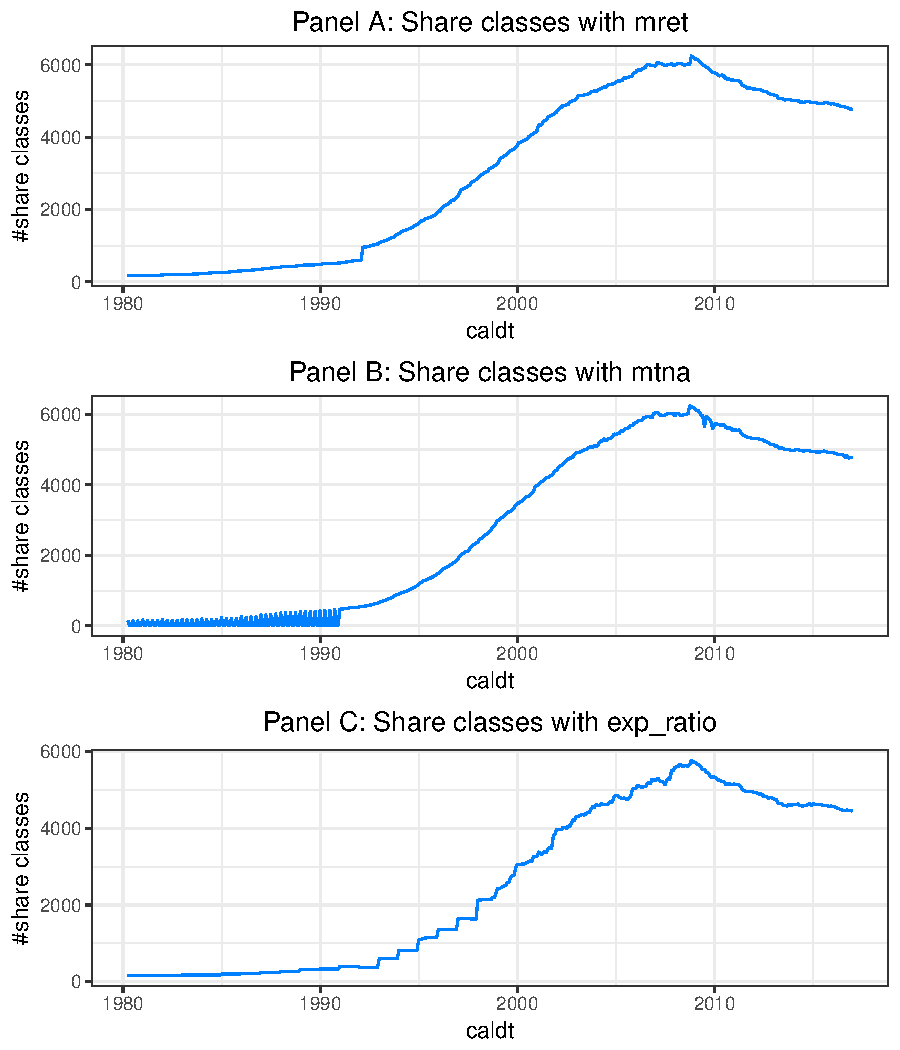
\includegraphics{appendix-summary_files/figure-latex/sampleCompleteness-1.pdf}
\caption{\label{fig:sampleCompleteness}Data Availability in the CRSP Mutual
Fund Dataset. Number of share class level observations passing filters
for identifying actively managed domestic equity funds. Note that
consistent mtna records begin January 1991. Further, there were over 300
share classes added to the dataset in Jan 1991, whose returns come
online Feb 1992. However, these added share classes do not have size and
expense ratio information, so do not majorly influence the fund level
dataset used in the analysis.}
\end{figure}

\begin{figure}
\centering
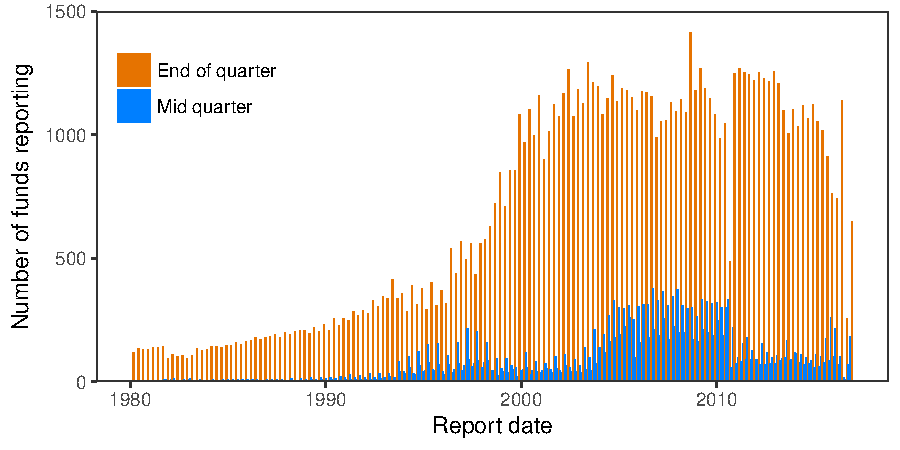
\includegraphics{appendix-summary_files/figure-latex/rdateFreq-1.pdf}
\caption{\label{fig:rdateFreq}Fund report dates in Thomson. Time series plot
of the number of funds reporting during a given month.}
\end{figure}

\begin{figure}
\centering
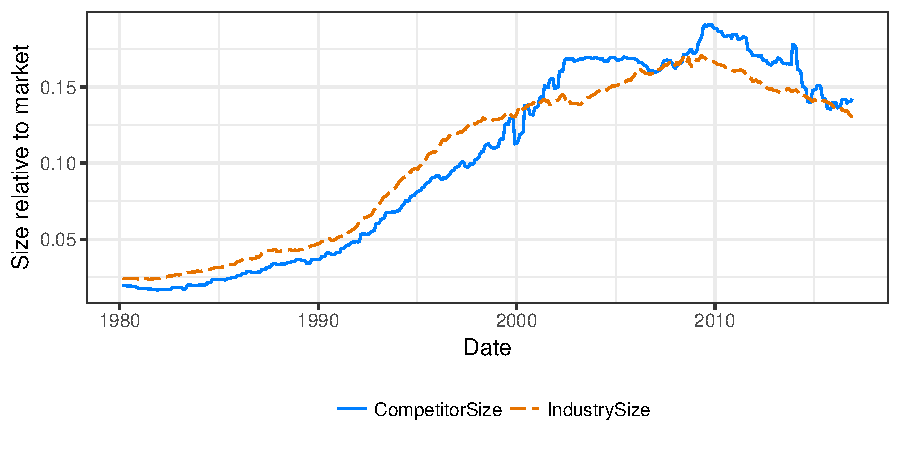
\includegraphics{appendix-summary_files/figure-latex/industrySize-1.pdf}
\caption{\label{fig:industrySize}Time series of \(CompetitorSize\).
Cross-sectional mean of \(CompetitorSize\) (scaled by 40 for exposition)
against the time series of \(IndustrySize\).}
\end{figure}

\hypertarget{sec:CSandPerformance}{%
\chapter{Competitor Size and Fund
Performance}\label{sec:CSandPerformance}}

\hypertarget{sec:benchmark}{%
\section{Benchmarking Returns}\label{sec:benchmark}}

Ideally, I would like to benchmark mutual fund returns by factors that
are both near costlessly tradeable for funds, and span dimensions of
risk that are of concern to investors. In the absence of such an ideal
benchmark, I employ the conventional option of benchmarking returns with
Fama-French factors. Define three factor benchmark adjusted gross
returns as \begin{equation}
R^{FF3}_{i,t} = R_{i,t} - \left[ \hat{\beta}^{RMRF}_i RMRF_t + \hat{\beta}^{SMB}_i SMB_t + \hat{\beta}^{HML}_i HML_t \right],
\end{equation} where \(R_{i,t}\) is the gross return of fund \(i\) at
month \(t\) in excess of the risk free rate, expressed in percentages.
\(RMRF\), \(SMB\), and \(HML\) are the usual market, size, and value
factors. The beta hats are the sample estimates of each fund's exposure
to the respective factors, estimated by fund level regressions of the
form \begin{equation}
R_{i,t} = \alpha_i + \beta^{RMRF}_i RMRF_t + \beta^{SMB}_i SMB_t + \beta^{HML}_i HML_t + \varepsilon_{i,t}.
\end{equation} Therefore,
\(R^{FF3}_{i,t} = \hat{\alpha}_i + \hat{\varepsilon}_{i,t}\), i.e.~each
period's benchmark adjusted returns are equal to the sum of the fund's
estimated gross alpha and the given month's residual from the
Fama-French time series regressions.

Benchmarking with a factor model has some shortcomings and advantages.
The long-short SMB and HML portfolios are not tradeable for mutual
funds. \citet{bvb15} argue that at each point in time the performance of
active funds ought to be measured against the returns of the lowest cost
passive funds readily available to retail investors. This is an
eminently sensible suggestion for studying funds' value added for retail
investors, but not an obviously superior method for testing whether fund
alpha is decreasing in competitor scale. \citet{cpz12} note that
Fama-French benchmarks imply nonzero alphas for a number of mainstream
passive benchmarks. My results are robust to following their suggestion
of benchmarking with index-based factors. Unlike self-designated
benchmarks, Fama-French factors are not gameable by funds. They are also
widely available.\footnote{As argued by \citet{pst15}, Morningstar
  benchmarks share the feature of non-gameability, but are proprietary.}
Unlike characteristic based benchmarks, factor based benchmarks are not
subject to errors in holdings data, are available monthly, and account
for the unobserved actions of funds. Lastly, regardless of whether size
and value correspond to risk, Fama-French factors capture a large
fraction of variance in cross-sectional returns.

\hypertarget{regression-setup}{%
\section{Regression Setup}\label{regression-setup}}

I implement within-fund regression specifications of the following form
to test for decreasing returns to competitor scale: \begin{equation}
R^{FF3}_{i,t+1} = \alpha_i + \gamma CompetitorSize_{i,t} + \mathbf{X}_{i,t}\Gamma + \varepsilon_{i,t+1},
\label{eq:regSpec}
\end{equation} where \(\alpha_i\) are firm fixed effects, and
\(\mathbf{X}_{i,t}\) is a vector of controls including \(IndustrySize\)
and year-month fixed effects.\footnote{Since \(IndustrySize\) only
  varies in the time series, it is omitted in regressions featuring
  year-month fixed effects. Similarly, \(FundAge\) is fully absorbed by
  the combination of fund and year-month fixed effects.} The coefficient
of interest is \(\gamma\). To make the economic magnitude of the
coefficient easier to interpret, I annualize returns and divide
\(CompetitorSize\) and \(IndustrySize\) by their respective standard
deviations before performing the regressions. I re-scale \(FundSize\) by
the difference between the 50\(^\text{th}\) and 10\(^\text{th}\)
percentiles of its distribution.

I include fund fixed effects throughout to take into account the
possibility that baseline fund skill and average competitor size are
related in the cross-section, i.e.
\(\text{Cov}(\alpha_i, \overline{CompetitorSize}_i)\neq 0\). We would
expect talented managers to be endogenously allocated where they are
most capable of taking advantage of investment opportunities. Bolstering
this view, \citet{bbl17} show that fund families funnel capital toward
skilled managers. A mechanical concern is that in the cross-section
\(CompetitorSize\) tends to be higher for funds in large cap sectors.
Since more liquid market segments can absorb a larger amount of active
investment, not all cross-sectional variation of \(CompetitorSize\)
reflects variation in the effective inter-fund competition for
investment opportunities. Controlling for fund fixed effects is a
parsimonious way of controlling for such fixed differences in funds'
operating environment.

For the specifications including fund fixed effects only, deviations of
\(CompetitorSize\) from its within-fund mean provide the variation
identifying the coefficient of interest. For regressions including both
fund and year-month fixed effects, the coefficient of interest is
identified based on deviations of \(CompetitorSize\) from its
within-fund mean, relative to the average within-fund deviation at each
date. Year-month fixed effects control nonparametrically for common time
series variation in returns and industry competition, ruling out the
possibility that the identified effect of competitor size is an artifact
of other aggregate developments, such as shared time-varying exposure to
competition from hedge funds. However, including overly fine
cross-sectional dummy variables would risk soaking up the variation of
interest.

I include \(IndustrySize\) to demonstrate that \(CompetitorSize\)
captures distinct variation in decreasing returns faced by funds.
Controlling for \(FundSize\) is relevant for separating industry-level
decreasing returns to scale from fund-level decreasing returns to
scale.\footnote{Interpreting the coefficient on \(FundSize\) is
  problematic in within-fund regressions of returns. To be unbiased,
  within-fund regressions require strict exogeneity of the regressors
  {[}\citet{chamberlain82}; stambaugh99{]}, meaning
  \(\text{Cov}(x_{i,t},\varepsilon_{i,s})=0 \ \forall s\in\{1,2,\ldots,T_i\}\).
  Since past idiosyncratic high (low) returns mechanically increase
  (decrease) total net assets, we will typically have
  \(\text{Cov}(FundSize_{i,t},\varepsilon_{i,s})>0\) for \(s<t\), and a
  downward bias in the estimated coefficient. In simulations,
  \citet{hl17} estimate the bias around 14\%. \citet{pst15} propose a
  recursive demeaning (RD) procedure for eliminating this bias. The
  point estimates they report with the RD procedure are similar to those
  from the fixed effects OLS regressions, but the standard errors
  increase almost twenty-fold. Given that estimating the magnitude of
  decreasing returns to own size is not the focus of this study and the
  unfavorable tradeoff between bias and variance, I choose to not
  implement the RD procedure.}

For constructing standard errors, each month I sort funds into ten
mutually exclusive (but not necessarily equal sized) portfolio groups
based on their most recently reported holdings.\footnote{Funds are
  grouped using k-means cluster analysis of raw portfolio weights. Each
  month, this process constructs \(k=10\) archetypal portfolios (serving
  as cluster centers). These model portfolios are constructed and then
  funds are assigned to them such that the sum of squared differences
  between the weights of fund portfolios and their assigned model
  portfolio is minimized.} I double cluster standard errors by fund and
year-month \(\times\) portfolio group, to account for both within-fund
and cross-sectional correlation in errors. In practice, I find that
clustering by fund in regressions of returns is essentially irrelevant,
as within-fund correlation in the error term is negligible. On the other
hand, the cross-sectional correlation structure of regression errors is
substantive. The number of portfolio groups is similar to the number of
Morningstar sectors. Each month's largest portfolio group cluster on
average accounts for over a third of observations. Therefore, portfolio
group \(\times\) month clusters allow for extensive within month
correlation of errors, without reducing the number of clusters
unreasonably.

\hypertarget{results-1}{%
\section{Results}\label{results-1}}

Table \ref{tab:mainResults} presents results from the equation
\eqref{eq:regSpec} regression specifications. There is a consistently
negative, statistically significant within fund relation between
\(CompetitorSize\) and fund performance. Coefficients range from -1.06
in the univariate within-fund regression to -0.78 in the specification
featuring the full set of fund and year-month fixed effects and own
size. While \(IndustrySize\) is associated with a statistically
significant -0.39 coefficient in the specification with no other
controls (column (2)), adding \(CompetitorSize\) to the specification
(column (3)) subsumes its negative effect, with the coefficient on
\(IndustrySize\) dropping to an insignificant 0.10. Although
coefficients associated with own fund size are consistently negative and
statistically significant, they are known to be biased and should be
interpreted with caution.\footnote{Consistent with \citet{hl17}, I find
  much larger estimates of decreasing returns to own size when using a
  log transform of \(FundSize\).}

\label{tab:mainResults}Decreasing Returns to Competitor Scale The regression
sample contains actively managed domestic equity mutual funds from 1980
to 2016. The dependent variable is three-factor adjusted gross returns,
in annualized percentages. Size variables are as defined in Section
\ref{sec:CompetitorSize}. \(CompetitorSize\) and \(IndustrySize\) are
normalized by their respective sample standard deviations. \(FundSize\)
is normalized by the difference between the 50th and 10th percentile of
its distribution. Each fund is assigned to one of ten portfolio group
clusters each month based on k-means clustering of most recent portfolio
holdings. Standard errors are double clustered by fund and year-month
\(\times\) portfolio group, and reported in parentheses. Asterisks
denote statistical significance: \(\ast\ast\ast\) p\$

\left(1\right)

\left(2\right)

\left(3\right)

\left(4\right)

\(CompetitorSize\)

-0.983***

-1.059***

-0.775***

(0.178)

(0.225)

(0.142)

\(IndustrySize\)

-0.392**

0.097

(0.178)

(0.224)

\(FundSize\)

-0.024***

(0.009)

Fixed Effects

\(\bullet\) Fund

Yes

Yes

Yes

Yes

\(\bullet\) Month

No

No

No

Yes

Observations

363,203

363,203

363,203

363,203

\(R^2\)

0.012

0.012

0.012

0.102

\(R^2\) (proj. model)

0.001

0.000

0.001

0.001

Expense ratios provide an informative comparison for the magnitude of
the \(CompetitorSize\) coefficients. The mean expense ratio in my sample
is 1.23\% per year, with an interquartile range of 0.49\%. A one
standard deviation increase in \(CompetitorSize\) is associated with a
drop in performance on the order of two thirds the typical fund expense
ratio. Decreasing returns to competitor scale are a meaningful
impediment to sustainable profitable operations for funds.

\hypertarget{sec:heterogeneity}{%
\section{The Role of Portfolio Liquidity}\label{sec:heterogeneity}}

Economic reasoning dictates that decreasing returns to competitor scale
operate through the price impact of competing funds. Therefore, we would
expect decreasing returns to be more severe for funds relying on less
liquid strategies. I test this by comparing the magnitude of decreasing
returns across funds with different levels of average portfolio
liquidity. Specifically, I run regressions of the form \begin{align}
\begin{split}
R^{FF3}_{i,t+1} = \alpha_i + \alpha_t &+ \gamma_1 CompetitorSize_{i,t} + \gamma_2 \left( CompetitorSize_{i,t} \times \overline{PortLiq}_{i} \right) \\ 
&+ \eta_1 FundSize_{i,t} + \eta_2 \left( FundSize_{i,t} \times \overline{PortLiq}_i \right) + \varepsilon_{i,t+1},
\end{split}
\label{eq:AvgLiqReg}
\end{align} where \(\overline{Port.Liq}_i\) is either the fund-level
average portfolio liquidity measure proposed by \citet{pst17L}, or any
of its sub-components of stock liquidity (average relative market
capitalization of holdings), coverage (number of stocks held relative to
total stocks in the market), and balance (a measure of how closely
portfolio weights track market weights of stocks in the portfolio).
Diversification is the product of coverage and balance. I re-scale each
variable so that a unit increase corresponds to the interquartile range
of within-fund means. If decreasing returns to scale are rooted in
liquidity constraints, we expect \(\gamma_2>0\).

Panel A of Table \ref{tab:roleOfLiquidity} presents results from the
regressions. All \(\gamma_2\) coefficients are positive and three out of
five are statistically significant. The economic magnitudes are large as
well. Increasing average portfolio liquidity from the
25\textsuperscript{th} to the 75\textsuperscript{th} percentile of its
distribution changes the impact of a one standard deviation increase in
\(CompetitorSize\) by 0.23bp in annualized returns. Decomposing
portfolio liquidity into its components demonstrates that the majority
of the effect is attributable to stock liquidity, with a lesser amount
attributable to diversification, including coverage and
balance.\footnote{In unreported results, I find a similar pattern of
  more severe decreasing returns for funds employing less liquid
  strategies using ad hoc measures of portfolio liquidity such as the
  portfolio-weighted average market weight of holdings, number of stocks
  held, share of largest five holdings, the Herfindahl-Hischman Index of
  portfolio weights, as well as own size and turnover.}

\label{tab:roleOfLiquidity}The Role of Portfolio Liquidity The dependent
variable is three-factor adjusted gross returns, in annualized
percentages. Size variables are normalized according to the Table
\ref{tab:mainResults} caption. \(L\), \(S\), \(D\), \(C\), \(B\) are
portfolio liquidity, stock liquidity, diversification, coverage, and
balance, as defined in \citet{pst17L}. \(\bar{L}\), \(\bar{S}\),
\(\bar{D}\), \(\bar{C}\), \(\bar{B}\) denote fund-level means. \(X\)
variables are normalized by interquartile range. Each fund is assigned
to one of ten portfolio group clusters each month based on k-means
clustering of most recent portfolio holdings. Standard errors are double
clustered by fund and year-month \(\times\) portfolio group, and
reported in parentheses. Asterisks denote statistical significance:
\(\ast\ast\ast\) p\$

\(X=\)

\(L\)

\(S\)

\(D\)

\(C\)

\(B\)

Panel A: Fund Level Average Portfolio Liquidity

\(Comp.Size \times \bar{X}\)

0.232***

0.324

0.048***

0.068***

0.308

(0.075)

(0.279)

(0.017)

(0.020)

(0.191)

\(FundSize \times \bar{X}\)

0.028***

0.010

0.006**

0.004*

0.005

(0.010)

(0.022)

(0.003)

(0.002)

(0.015)

\(CompetitorSize\)

-1.189***

-1.089***

-0.869***

-0.934***

-1.287***

(0.207)

(0.309)

(0.152)

(0.162)

(0.359)

\(FundSize\)

-0.075***

-0.030

-0.034***

-0.036***

-0.032

(0.021)

(0.022)

(0.011)

(0.013)

(0.027)

Fixed Effects

\(\bullet\) Fund

Yes

Yes

Yes

Yes

Yes

\(\bullet\) Month

Yes

Yes

Yes

Yes

Yes

Observations

363,203

363,203

363,203

363,203

363,203

\(R^2\)

0.103

0.102

0.102

0.102

0.102

\(R^2\) (proj. model)

0.001

0.001

0.001

0.001

0.001

Panel B: Real Time Portfolio Liquidity

\(Comp.Size \times X\)

0.159***

-0.240

0.039**

0.057***

0.421***

(0.041)

(0.246)

(0.019)

(0.020)

(0.130)

\(FundSize \times X\)

0.008**

0.002

0.011***

0.006**

0.015**

(0.004)

(0.008)

(0.002)

(0.003)

(0.007)

\(X\)

-0.737**

-1.032*

-0.046

0.037

-1.681***

(0.302)

(0.566)

(0.091)

(0.067)

(0.283)

\(CompetitorSize\)

-0.887***

-0.474*

-0.905***

-0.968***

-1.102***

(0.204)

(0.266)

(0.157)

(0.164)

(0.287)

\(FundSize\)

-0.050***

-0.026**

-0.052***

-0.043***

-0.048***

(0.014)

(0.013)

(0.010)

(0.012)

(0.015)

Fixed Effects

\(\bullet\) Fund

Yes

Yes

Yes

Yes

Yes

\(\bullet\) Month

Yes

Yes

Yes

Yes

Yes

Observations

363,203

363,203

363,203

363,203

363,203

\(R^2\)

0.103

0.103

0.102

0.103

0.103

\(R^2\) (proj. model)

0.001

0.001

0.001

0.001

0.001

A related question is whether funds can actively ameliorate the
pernicious effects of decreasing returns to (competitor) scale by
choosing more liquid portfolios. I test this by replacing fund-level
average measures of portfolio liquidity in equation \eqref{eq:AvgLiqReg}
with real time values: \begin{align}
\begin{split}
R^{FF3}_{i,t+1} = \alpha_i + \alpha_t &+ \gamma_1 CompetitorSize_{i,t} + \gamma_2 \left( CompetitorSize_{i,t} \times PortLiq_{i,t} \right) \\ 
&+ \eta_1 FundSize_{i,t} + \eta_2 \left( FundSize_{i,t} \times PortLiq_{i,t} \right)  \\
&+\gamma_3 PortLiq_{i,t} + \varepsilon_{i,t+1}.
\end{split}
\end{align} Panel B of Table \ref{tab:roleOfLiquidity} presents results
from the regressions. With the exception of stock liquidity, the
interaction terms are all positive and statistically significant,
suggesting that increased portfolio liquidity shelters the fund from
decreasing returns to scale. Note that the main effect of portfolio
liquidity is negative, suggesting that funds make more when they hold
more concentrated portfolios. This is consistent with funds responding
to time-varying investment opportunities by decreasing portfolio
liquidity when expected returns are high.

\bibliography{mf\_references.bib}


\end{document}
